%%%%%%%% ICML 2022 EXAMPLE LATEX SUBMISSION FILE %%%%%%%%%%%%%%%%%

\documentclass{article}

% Recommended, but optional, packages for figures and better typesetting:
\usepackage{microtype}
\usepackage{graphicx}
\usepackage{subfigure}
\usepackage{booktabs} % for professional tables
\usepackage{amsmath}
\usepackage{amsfonts}
\usepackage{multirow}
\usepackage{accents} 

\usepackage{ntheorem}
\theoremseparator{:}
\newtheorem{hyp}{Assumption}

\usepackage{tikz}
\usetikzlibrary{positioning,shapes,arrows}
% hyperref makes hyperlinks in the resulting PDF.
% If your build breaks (sometimes temporarily if a hyperlink spans a page)
% please comment out the following usepackage line and replace
% \usepackage{icml2021} with \usepackage[nohyperref]{icml2021} above.
\usepackage{hyperref}

% Attempt to make hyperref and algorithmic work together better:
\newcommand{\theHalgorithm}{\arabic{algorithm}}
\newcommand\figref{Figure~\ref}
\newcommand\Cref{Table~\ref}
\newcommand\appref{Appendix~\ref}
\newcommand\hypref{A\ref}
\newcommand\secref{Section~\ref}

\usepackage[accepted]{icml2022}
\icmltitlerunning{Robust Hybrid Learning With Expert Augmentation}

\begin{document}

\twocolumn[
\icmltitle{Robust Hybrid Learning With Expert Augmentation
}

\icmlsetsymbol{equal}{*}

\begin{icmlauthorlist}
\icmlauthor{Antoine Wehenkel}{to,apple_intern}
\icmlauthor{Jens Behrmann}{apple}
\icmlauthor{Hsiang Hsu}{harvard,apple_intern}
\icmlauthor{Guillermo Sapiro}{apple}
\icmlauthor{Gilles Louppe}{to}
\icmlauthor{Jörn-Henrik Jacobsen}{apple}
\end{icmlauthorlist}

\icmlaffiliation{to}{University of Liege}
\icmlaffiliation{apple}{Apple}
\icmlaffiliation{apple_intern}{Work done as an intern at Apple}
\icmlaffiliation{harvard}{Harvard University}

\icmlcorrespondingauthor{Antoine Wehenkel}{antoine.wehenkel@uliege.be}
\icmlkeywords{Machine Learning, ICML}

\vskip 0.3in
]
\printAffiliationsAndNotice{\icmlEqualContribution} 


\begin{abstract}
Hybrid modelling reduces the misspecification of expert models by combining them with machine learning (ML) components learned from data. Like for many ML algorithms, hybrid model performance guarantees are limited to the training distribution. Leveraging the insight that the expert model is usually valid even outside the training domain, we overcome this limitation by introducing a hybrid data augmentation strategy termed \textit{expert augmentation}. Based on a probabilistic formalization of hybrid modelling, we show why expert augmentation improves generalization. Finally, we validate the practical benefits of augmented hybrid models on a set of controlled experiments, modelling dynamical systems described by ordinary and partial differential equations. 
\end{abstract}

%%%%%%%%%%%%%%%%%%%%%%%%%%%%%%%%%% 1 INTRODUCTION %%%%%%%%%%%%%%%%%%%%%%%%%%%%%%%%%%
\section{Introduction}
Generalization to unseen data is a key property of a useful model. When training and test data are independently and identically distributed~(IID), one way to check generalization is by evaluating the model on a held out subset of the training data or with k-fold cross validation. Unfortunately, this setting is often unrealistic because the training scenario is rarely fully representative of the test scenario. This has motivated lot of recent research efforts to focus on  the robustness of ML models  \citep{gulrajani2020search,geirhos2020shortcut,koh2021wilds}. Common strategies can be broadly grouped in two categories: The first class of methods aims at aligning specific properties of the model (e.g., invariance, equivariance, monotonicity, etc.) with expertise on the problem of interest \citep{cubuk2019autoaugment, graph_net_molecule, universal_equivariance, alphago}. The second category is data focused \citep{groupDRO_ICLR, IRM, krueger2021out, creager2021environment} and leverages variations present in the training data, e.g. by minimizing worst case sub-group performance, to achieve robustness.

\begin{figure}[t]
    \centering
    \vspace{-.5em}
    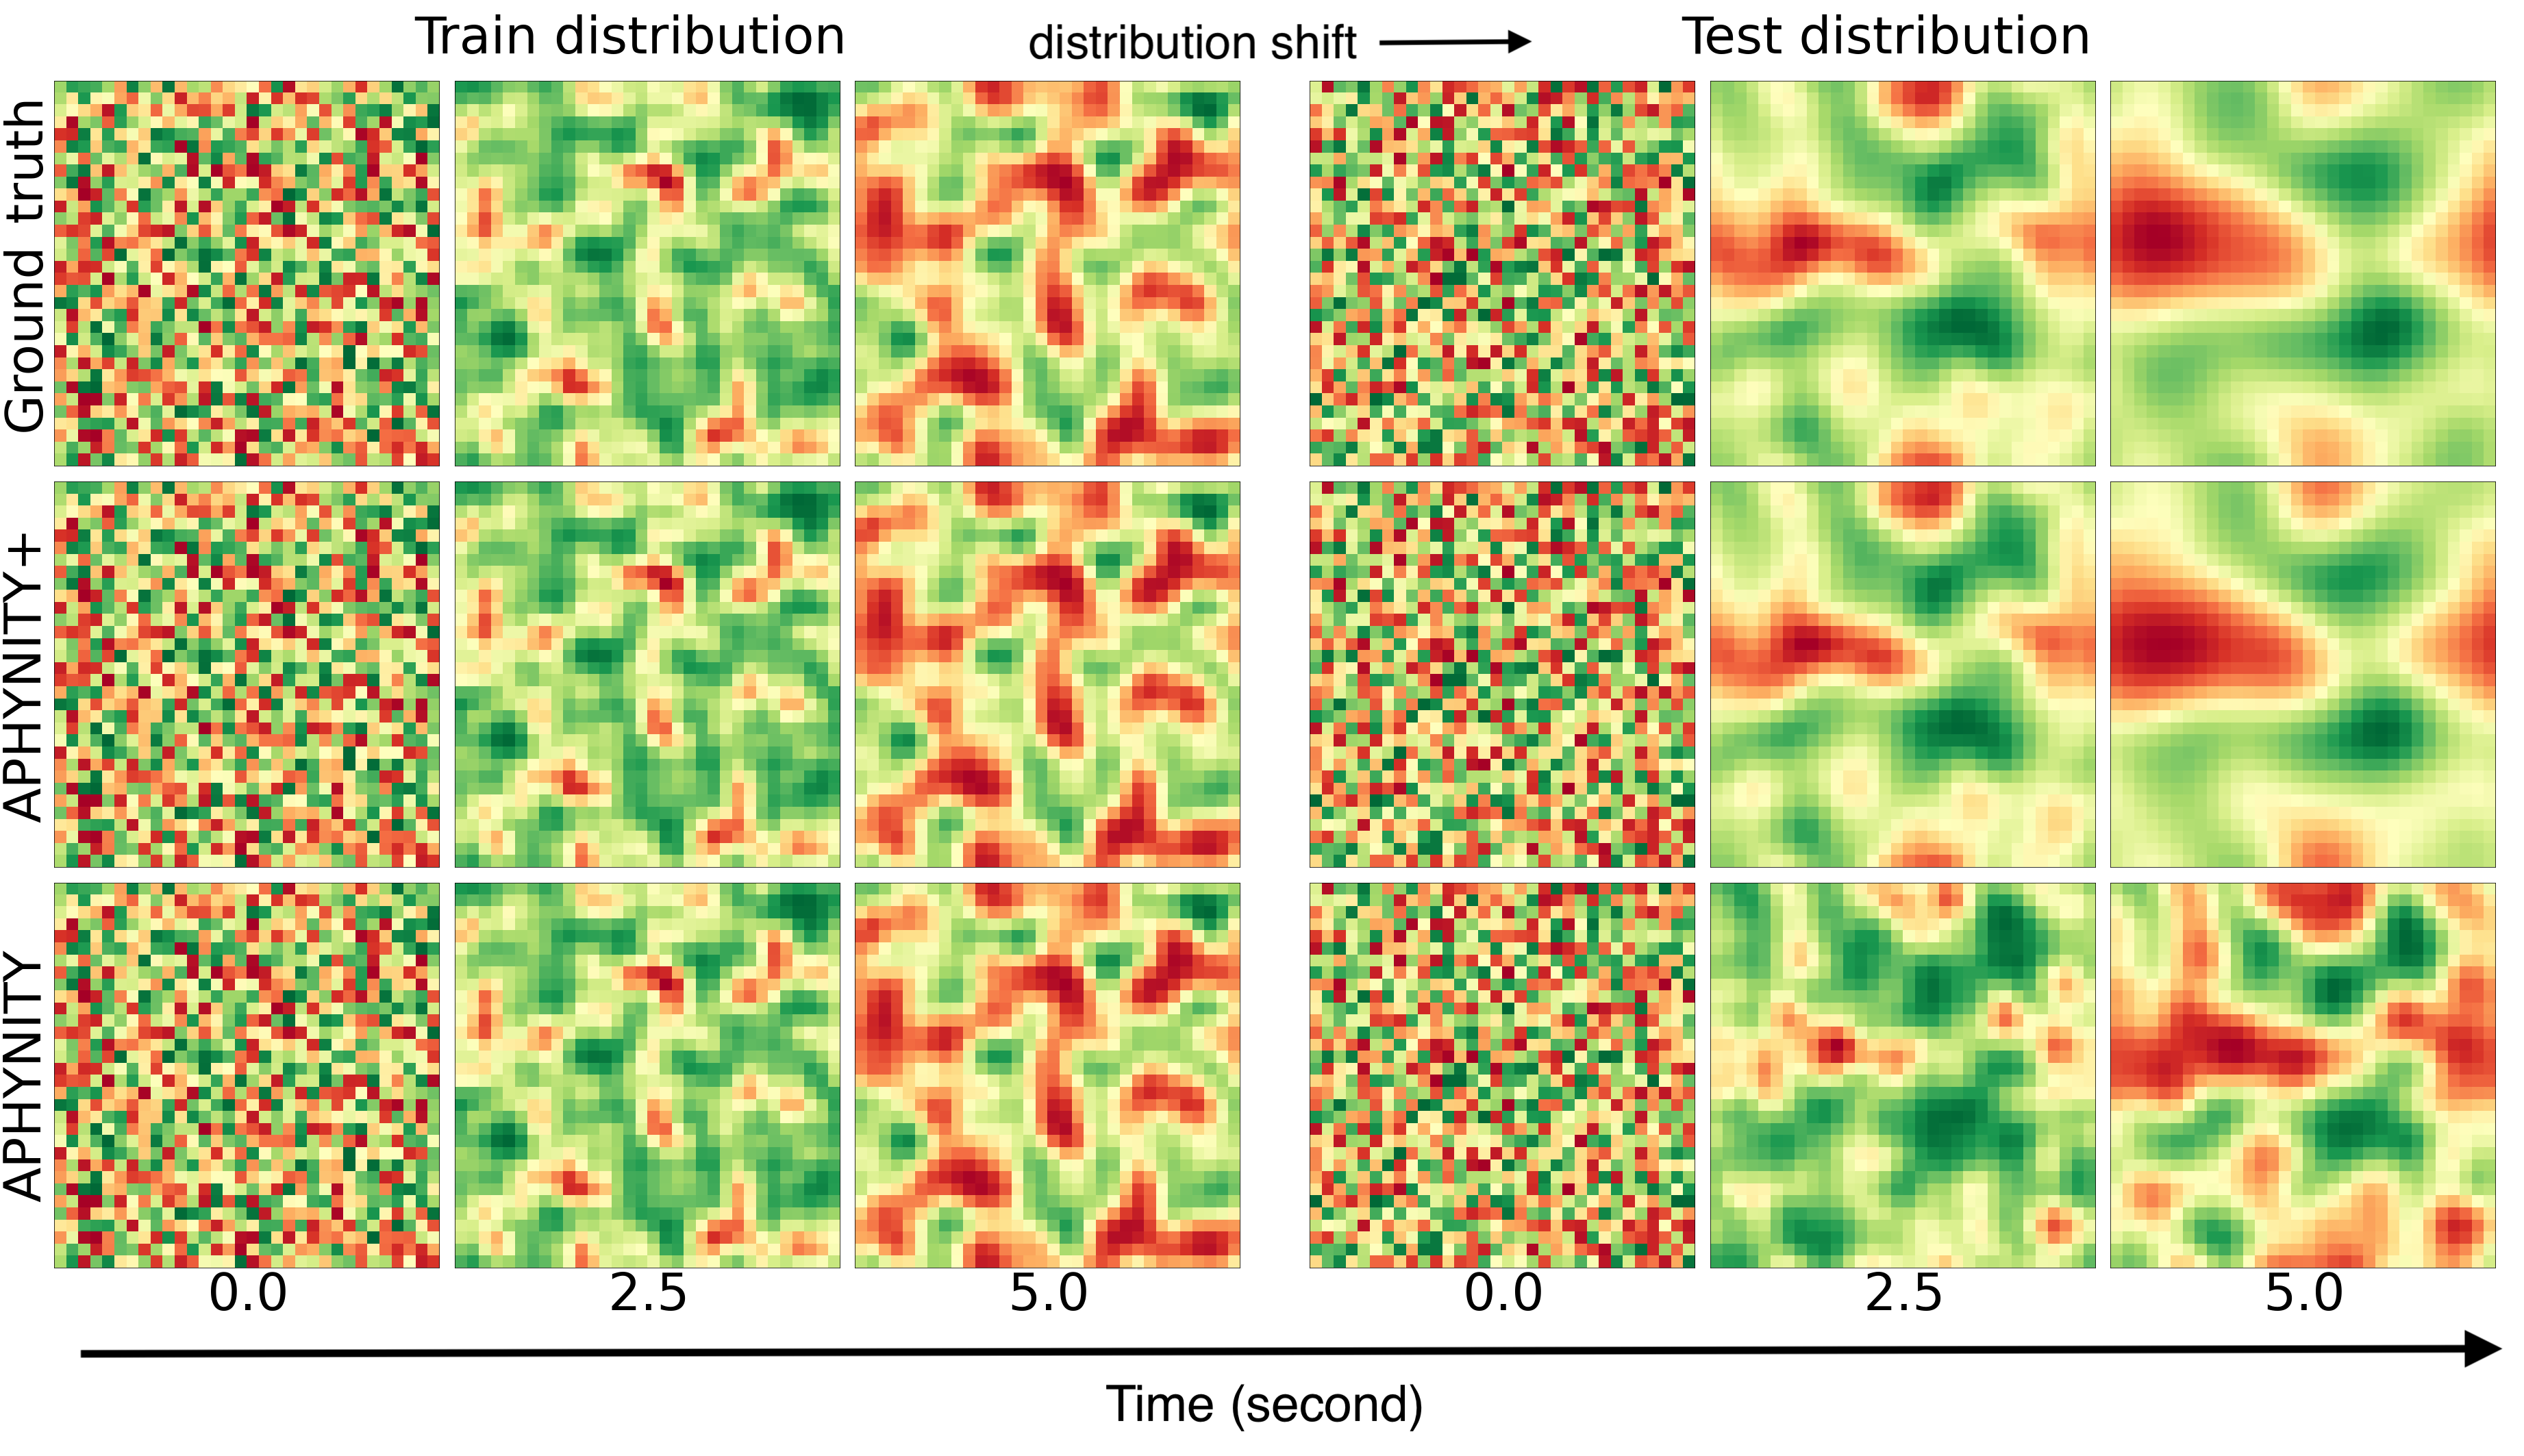
\includegraphics[width=.49\textwidth]{figures/improved_diffusion.png}
    \vspace{-2.em}
    \caption{APHYNITY, an existing hybrid modelling strategy, is unable to predict accurately the dynamic of a 2D diffusion reaction for a shifted test distribution although it predicts well configuration that follows the training distribution. On the opposite, APHYNITY+, the same model fine-tuned with our data augmentation, generalizes to shifted distributions as expected from the validity of the underlying physics.}
    \label{fig:diffusion_shift}
    \vspace{-1em}
\end{figure}

The data oriented methods, which include Group-DRO~\citep{groupDRO_ICLR} and Invariant Risk Minimization~\citep[][IRM]{IRM}, can be very appealing because they only require implicit specification of invariances via domains or environments. However, these methods' performance is limited to variations present in the training data and the inductive bias of the ML algorithm. This may be insufficient when the modelling problem is too complex or the variations of interest are not present in the training data. On the other hand, methods based on domain-specific expertise do not suffer from such limitations. Embedding expertise into a model can be done via architectural inductive biases \citep{lecun_cnn, gnn}, data augmentation \citep{cubuk2019autoaugment}, or a learning objective \citep{lagrangian_nn} that enforces established symmetries of the problem. As an example, simple data augmentation techniques combined with convolutions lead to excellent performance on natural image problems \citep{cubuk2019autoaugment}. Another natural approach to embed expertise in ML models, and the one studied in this paper, is called hybrid learning (HyL). HyL combines an expert model (e.g., physics-motivated equations) with a learned component that improves the expert model so that the combination better fits real-world data. A particularity of HyL is the central role played by the expertise, which is supposed to provide a simple and well-grounded parametric description of the process considered. HyL usually considers the expert model as an analytical function, or as a set of equations, that relates the expert parameters to the quantity of interest. The expert model is often motivated by the underlying physics of the system considered. Hence, we will use the terms \textit{expert} model and \textit{physical} model interchangeably.

In recent work \citep{APHYNITY, HVAE, latent_ode_pharma, hl_1, hl_2, hl_3}, HyL demonstrated success in complementing partial physical models and improving the inference of the corresponding parameters. However, contrarily to the common belief that HyL achieves better generalization than black box ML models, we argue that hybrid models do not meet their promise regarding robustness. Although HyL achieves strong performance on IID test distributions by exploiting the inductive bias of the expert models, we show that their performance collapses when the test domain is not included in the training domain. This is unsatisfactory as the expert model is typically well-defined for a range of parameters that can correspond to realistic data far outside of the training distribution. A test distribution not covered by the training data, but for which an expert model exists, happens often in the real world. As an example, \citet{latent_ode_pharma} apply HyL to a pharmacological model describing the effect of a COVID-19 treatment for which only a limited quantity of real-world data is available. In this context, although the underlying biochemical dynamic of treatments is well modelled, data is often scarce and biased. Therefore, the hybrid model does not necessarily generalize to configurations that are well modelled by the pharmacological model but unseen during training.

We introduce \textit{expert augmentations} for training augmented hybrid models~(AHMs), a procedure that extends the range of validity of hybrid models and improves generalization as pictured by \figref{fig:diffusion_shift}. Our contribution is to first formalise the HyL problem as: 1) Learning a probabilistic model partially defined by the expert model; 2) Performing inference over this probabilistic hybrid model. In this context, we show that HyL is vulnerable to distribution shifts for which the expert model is well defined (see Figure \ref{fig:diffusion_shift}, bottom row). Motivated by our analysis, we propose to fine-tune the hybrid model on an expert-augmented dataset that includes distribution shifts (see results of augmentation in Figure \ref{fig:diffusion_shift}, middle row). These expert augmentations only rely on the hybrid model itself, leveraging that the expert model is also well-defined outside of the training distribution. Our experiments on various controlled HyL problems demonstrate that AHMs achieve multiple orders of magnitude superior generalization in realistic situations and can be applied to any state-of-the-art HyL algorithm.

%%%%%%%%%%%%%%%%%%%%%%%%%%%%%%%%%% 2 Hybrid learning %%%%%%%%%%%%%%%%%%%%%%%%%%%%%%%%%%
\section{Hybrid learning}
\begin{figure}
    \centering
    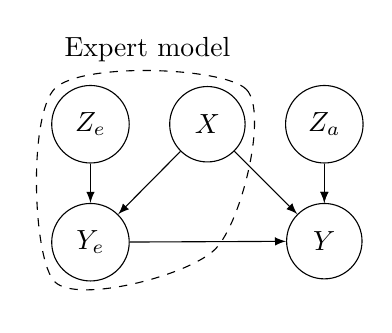
\begin{tikzpicture}[
          node distance=.5cm and .5cm,
          mynode/.style={draw,circle,text width=.6cm,align=center},
          phantom_node/.style={circle,text width=.6cm,align=center},
          halo/.style={line join=round,
          double,line cap=round,double distance=#1,shorten >=-#1/2,shorten <=-#1/2},
          halo/.default=7mm]
        \node[mynode] (zp) {$Z_e$};
        \node[mynode, right=of zp] (x) {$X$};
        \node[mynode, right=of x] (za) {$Z_a$};
        \node[mynode, below=of zp] (yp) {$Y_e$};
        \node[mynode, below=of za] (y) {$Y$};
        \path (zp) edge[-latex] (yp);
        \path (x) edge[-latex] (yp);
        \path (x) edge[-latex] (y);
        \path (yp) edge[-latex] (y);
        \path (za) edge[-latex] (y);
        \path (za) edge[-latex] (y);
        
        \coordinate (A) at ([yshift=.1cm,xshift=-.1cm]zp.north west);
        \coordinate (B) at ([yshift=.1cm,xshift=.15cm]x.north east);
        \coordinate (C) at ([xshift=-.1cm,yshift=-.15cm]yp.south west);
        \coordinate (D) at ([yshift=-1.1cm,xshift=.1cm]x.south);
        
        \coordinate (A_right) at ([yshift=.5cm,xshift=0cm]A);
        \node at (A_right) [right] {Expert model};

        \draw[dashed] plot[smooth cycle] coordinates {(A) (B) (D) (C)};

        
    \end{tikzpicture}
    \caption{A hybrid probabilistic model which describes the relationship between the input $X$ and the output $Y$ for a configuration of the system as defined by the latent variables $Z_e$ and $Z_a$. The prescribed expert model defines the conditional density $p(y_e|z_e, x)$, where $Y_e$ is an approximation of $Y$. Hybrid learning aims at learning the conditional distribution $p(y|z_a, y_e, x)$.}
    \label{fig:gen_bnet}
    \vspace{-1em}
\end{figure}

In order to show that our proposed expert augmentations lead to robust models, we first formalize hybrid learning with the probabilistic model depicted in \figref{fig:gen_bnet}. In this Bayesian network, capital letters denote random variables (e.g., $Y$) and, in the following, we will use calligraphic letters for the domain of the corresponding realization (e.g., $y \in \mathcal{Y}$). In our formalism, the expert model is a conditional density $p(y_e|x, z_e)$ that describes the distribution of the $expert$ response $Y_e$ to an input $x$ together with a parametric description of the system $z_e$, denoting expert or physical parameters. We augment the expert model with the \textit{interaction model} which is a conditional distribution $p(y|x, y_e, z_a)$ that describes the distribution of the observation $Y$ given the input $x$, the expert model response $y_e$, and a parametric description of the interaction model $z_a$.

Our final goal is to create a robust predictive model $p(y|x, (x_o, y_o))$ of the random variable $Y$, given the input $x$ together with independent observations $(x_o, y_o)$ of the same system, where the subscript $o$ denotes an observed quantity. As a concrete example, we consider predicting the evolution of a damped pendulum (described in \secref{sec:problems_description}) given its initial angle and speed ($x = \left[ \theta, \dot\theta\right]$) and a sequence of observations of the same pendulum. The expert model we assume is able to describe a frictionless pendulum whose dynamic is only characterized by one parameter $z_e := \omega_0$, denoting its fundamental frequency. A perfect description of the system should model the friction with a second parameter $z_a := \alpha$, the damping factor. In this problem, $(x_o, y_o)$ and $(x, y)$ are IID realization of the same pendulum which corresponds, in general terms, to samples from $p(x, y|z_a, z_e)$ for some fixed but unknown values of $z_a$ and $z_e$. The expert variables $z_e$ (e.g., $\omega_0$) together with $z_a$ (e.g., $\alpha$) should accurately describe the system that produces $Y$ (e.g., the evolution of the pendulum's angle and speed along time) from $X$ (e.g., the initial pendulum's state). In our setting we assume that we are given a pair $(x_o, y_o)$ (e.g., past observations) from which we can accurately infer the state of the system $(z_a, z_e)$ as described by the interaction and expert models, and then predict the distribution of $Y$ for a given input $x$ (e.g., forecasting future observations) to the same system. Because the interaction between $z_e$ and $y$ is essentially defined by the expert model, it should be possible, and preferable, to learn an accurate predictive model of $Y$ whose accuracy is independent from the training distribution of the expert variables $z_e$. Provided all probability distributions in \figref{fig:gen_bnet} are known, the Bayes optimal hybrid predictor $p_B$ can be written as 
\begin{align}
    p_B(y|x, (x_o, y_o)) = \mathbb{E}_{p(z_a, z_e|(x_o, y_o))}\left[ p(y|x, z_a, z_e) \right]. \label{eq:hybrid_predictor}
\end{align}
We observe that the Bayes optimal predictor explicitly depends on the posterior $p(z_a, z_e|(x_o, y_o))$ which is itself a function of the marginal distribution over $z_e$. This may preclude the existence of a good predictor that is invariant to shift of $p(z_e)$. However, in the following we will consider that the pair $(x_o, y_o)$ contains enough information about the parameters $z_a, z_e$. As a consequence, the posterior distribution shrinks around the correct parameters value and the effect of the prior becomes negligible.


\subsection{Hybrid generative modelling}
We consider expert models that are deterministic; that is, for which $p_\theta(y_e|x, z_e)$ is a Dirac distribution. The expert model describes the system as a function $f_e : \mathcal{X} \times \mathcal{Z}_e \rightarrow \mathcal{Y}_e$ that computes the response $y_e$ to an input $x$, parameterized by expert variables $z_e$. The goal of hybrid modelling is to augment the expert model with a learned component from data as depicted in \figref{fig:gen_bnet}. Formally, given a dataset $\mathcal{D} = \{(x^{(i)}, y^{(i)})\}_{i=1}^N$ of $N$ IID samples, we aim to learn the interaction model $p_\theta(y|x, y_e, z_a)$ that fits the data well but is close to the expert model. For example, we could define closeness via a small L2-distance between expert and hybrid outputs or via a small Kullback-Leibler (KL) divergence between the marginal distributions of $Y$ and $Y_e$.

Learning a model that is close to the expert model and fits the training data well is a hard problem. However, the APHYNITY algorithm \citep{APHYNITY} and the Hybrid-VAE \citep[][HVAE]{HVAE} are two recent approaches that offer promising solutions to this problem. We now briefly describe these two methods and how they can be used to approximate the Bayes optimal predictor of \eqref{eq:hybrid_predictor}. Our augmentation strategy is compatible (and effective) with both approaches.
\paragraph{APHYNITY.}
\citet{APHYNITY} formulate hybrid learning in a context where the expert model is an ordinary differential equation (ODE). They consider an additive hybrid model that should perfectly fit the data, which is equivalent to assuming the conditional distribution $p_\theta(y|x, y_e, z_a)$ is a Dirac distribution. Formally, they solve the optimization problem
\begin{align}
    \min_{z_e, F_a} ||F_a|| \quad \text{s.t.} \quad \forall (x, y) \in \mathcal{D}, \forall t,& \frac{dy_t}{dt} = (F_e + F_a)(y_t) \nonumber \\ &\text{with} \quad y_0 := x, \label{eq:APHYNITY}
\end{align}
where $||\cdot||$ is a norm operator on the function space, $F_a: \mathcal{Y}_t \times \mathcal{Z}_a \rightarrow \mathcal{Y}_t$ is a learned function, $F_e: \mathcal{Y}_t \times \mathcal{Z}_e \rightarrow \mathcal{Y}_t$ defines the expert model and $\mathcal{D}$ is a dataset of initial states $x:=y_0$ and sequences $y \in \mathcal{Y} := (\mathcal{Y}_t)^k$, where $k$ is the number of observed timesteps. APHYNITY solves this problem with Lagrangian optimization and Neural ODEs~\citep{NODE} to compute derivatives. In the context of ODEs, the random variable $X$ is the initial state of the system at $t_0$ and $Y$ is the observed sequence of $k$ states between $t_0$ and $t_1$.

This formulation only considers learning a missing dynamic for one realization of the system described by \figref{fig:gen_bnet}, for a single $z_a$ and $z_e$. However, we are interested in learning a hybrid model that works for the full set of systems described by \figref{fig:gen_bnet}. As suggested in \citet{APHYNITY}, we use an encoder network $g_\psi(\cdot, \cdot): \mathcal{X} \times \mathcal{Y} \rightarrow \mathcal{Z}_a \times \mathcal{Z}_e$ that corresponds to a Dirac distribution located at $g_\psi$ as the approximate posterior $q_\psi(z_a, z_e|x, y)$. The interaction model is a product of Dirac distributions whose locations correspond to the solution of the ODE 
\begin{align}
    \frac{dy_t}{dt} = F_e(y_t, z_e) + F_a(y_t, z_a; \theta), \quad y_0:=x.
    \label{eq:APH_ae}
\end{align} 
Hence the corresponding approximate Bayes predictor replaces the parameters $(z_a, z_e)$ in \eqref{eq:APH_ae} with the prediction of $g_\psi$ and predicts a product of Dirac distributions.

\paragraph{Hybrid-VAE (HVAE).}
In contrast to APHYNITY, the model proposed by \citet{HVAE} is not limited to additive interactions between the expert model and the ML model, nor to ODEs. Instead, their goal is to learn the generative model described by \figref{fig:gen_bnet}. They achieve this with a variational auto-encoder (VAE) where the decoder specifically follows \figref{fig:gen_bnet}. Similarly to the amortized APHYNITY model, the encoder $g_\psi(x, y)$ predicts a posterior distribution over $z_a$ and $z_e$, and the model is trained with the classical Evidence Lower Bound on the likelihood~(ELBO). \citet{HVAE} observe that relying only on an architectural inductive bias and maximum likelihood training is not enough to ground the generative model to the expert equations. They propose to add three regularizers $R_{PPC}, R_{DA, 1},\text{ and } R_{DA, 2}$ that encourage the generative model to rely on the expert model. The final objective is 
\begin{align}
    \max_{\theta, \psi}\, &\mathbb{E}_{\mathcal{D}}\left[ \text{ELBO} ((x, y); \psi, \theta)\right] + \alpha R_{PPC} + \beta R_{DA, 1} \nonumber \\&+ \gamma R_{DA, 2}. \label{eq:hvae_loss}
\end{align}
The first regularizer, $R_{PPC}$, encourages the marginal distribution of samples generated by the complete model to be close to the marginal distribution that would be only generated by the physical model. The two other regularizers specifically require the encoder network for $z_e$ to be made of two sub-networks. The first network filters the observations to keep only what can be generated by the expert model alone, and the second should map the filtered observations to the posterior distribution over $z_e$. $R_{DA, 1}$ penalizes the objective if the observations generated by the expert model are not close to the filtered observations. Finally, $R_{DA, 2}$ relies on data augmentation with the expert model to enforce that the second sub-network correctly identifies the expert variables $z_e$ when the observations are correctly filtered. We refer the reader to \citet{HVAE} for more details on HVAE. For HVAE, the approximate predictor takes the form described by \eqref{eq:hybrid_predictor} where $p(z_a, z_e|(x_o, y_o))$ is approximated by the encoder $q_\psi(z_a, z_e|x, y)$ and $p(y|x, z_e, z_a)$ by the learned hybrid generative model.

\begin{figure*}[h]
    \centering
    \tikzset{every picture/.style={line width=0.5pt}} %set default line width to 0.75pt        

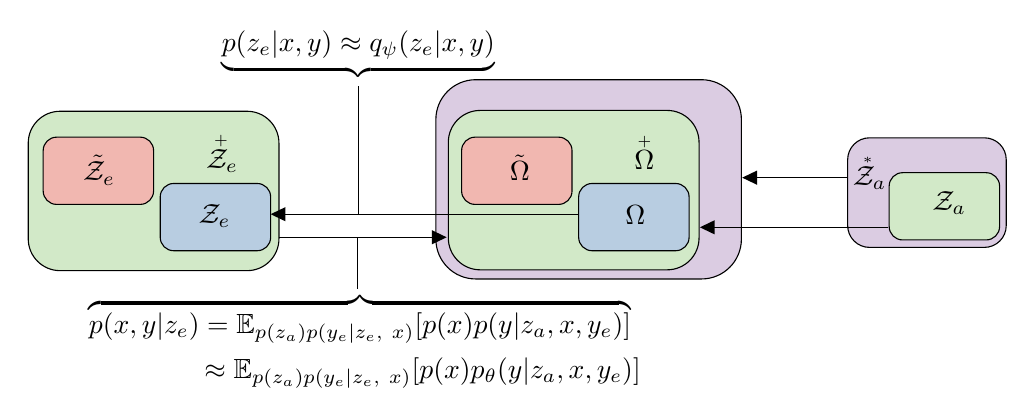
\begin{tikzpicture}[x=0.75pt,y=0.75pt,yscale=-1,xscale=1,scale=0.8]
%uncomment if require: \path (0,300); %set diagram left start at 0, and has height of 300

%All ALl omega
\draw  [color={rgb, 255:red, 0; green, 0; blue, 0 }  ,draw opacity=1 ][fill={rgb, 255:red, 219; green, 204; blue, 226 }  ,fill opacity=1. ] (247.5,65) .. controls (247.5,51.75) and (258.25,41) .. (271.5,41) -- (407.5,41) .. controls (420.75,41) and (431.5,51.75) .. (431.5,65) -- (431.5,137) .. controls (431.5,150.25) and (420.75,161) .. (407.5,161) -- (271.5,161) .. controls (258.25,161) and (247.5,150.25) .. (247.5,137) -- cycle ;

%All ze
\draw  [fill={rgb, 255:red, 210; green, 233; blue, 200 }  ,fill opacity=1. ] (2,79.2) .. controls (2,68.6) and (10.6,60) .. (21.2,60) -- (133.8,60) .. controls (144.4,60) and (153,68.6) .. (153,79.2) -- (153,136.8) .. controls (153,147.4) and (144.4,156) .. (133.8,156) -- (21.2,156) .. controls (10.6,156) and (2,147.4) .. (2,136.8) -- cycle ;
%all omega
\draw  [fill={rgb, 255:red, 210; green, 233; blue, 200 }  ,fill opacity=1. ] (255,78.7) .. controls (255,68.1) and (263.6,59.5) .. (274.2,59.5) -- (386.8,59.5) .. controls (397.4,59.5) and (406,68.1) .. (406,78.7) -- (406,136.3) .. controls (406,146.9) and (397.4,155.5) .. (386.8,155.5) -- (274.2,155.5) .. controls (263.6,155.5) and (255,146.9) .. (255,136.3) -- cycle ;

%Rounded Rect [id:dp6639592793786497] 
\draw [fill={rgb, 255:red, 241; green, 183; blue, 176 }  ,fill opacity=1. ]  (11,83.7) .. controls (11,79.23) and (14.63,75.6) .. (19.1,75.6) -- (69.4,75.6) .. controls (73.87,75.6) and (77.5,79.23) .. (77.5,83.7) -- (77.5,108) .. controls (77.5,112.47) and (73.87,116.1) .. (69.4,116.1) -- (19.1,116.1) .. controls (14.63,116.1) and (11,112.47) .. (11,108) -- cycle ;
%Rounded Rect [id:dp6448074412564562] 
\draw [fill={rgb, 255:red, 184; green, 205; blue, 225 }  ,fill opacity=1. ]  (81.5,111.6) .. controls (81.5,107.13) and (85.13,103.5) .. (89.6,103.5) -- (139.9,103.5) .. controls (144.37,103.5) and (148,107.13) .. (148,111.6) -- (148,135.9) .. controls (148,140.37) and (144.37,144) .. (139.9,144) -- (89.6,144) .. controls (85.13,144) and (81.5,140.37) .. (81.5,135.9) -- cycle ;

%Rounded Rect [id:dp7160429142184185] 
\draw  [fill={rgb, 255:red, 241; green, 183; blue, 176 }  ,fill opacity=1. ]  (263,83.7) .. controls (263,79.23) and (266.63,75.6) .. (271.1,75.6) -- (321.4,75.6) .. controls (325.87,75.6) and (329.5,79.23) .. (329.5,83.7) -- (329.5,108) .. controls (329.5,112.47) and (325.87,116.1) .. (321.4,116.1) -- (271.1,116.1) .. controls (266.63,116.1) and (263,112.47) .. (263,108) -- cycle ;
%Rounded Rect [id:dp8333286965822135] 
\draw [fill={rgb, 255:red, 184; green, 205; blue, 225 }  ,fill opacity=1. ]  (333.5,111.6) .. controls (333.5,107.13) and (337.13,103.5) .. (341.6,103.5) -- (391.9,103.5) .. controls (396.37,103.5) and (400,107.13) .. (400,111.6) -- (400,135.9) .. controls (400,140.37) and (396.37,144) .. (391.9,144) -- (341.6,144) .. controls (337.13,144) and (333.5,140.37) .. (333.5,135.9) -- cycle ;

\draw  [color={rgb, 255:red, 0; green, 0; blue, 0 }  ,draw opacity=1 ][fill={rgb, 255:red, 184; green, 233; blue, 134 }  ,fill opacity=0.3 ][fill={rgb, 255:red, 219; green, 204; blue, 226 }  ,fill opacity=1. ]  (495.5,89.2) .. controls (495.5,81.91) and (501.41,76) .. (508.7,76) -- (577.8,76) .. controls (585.09,76) and (591,81.91) .. (591,89.2) -- (591,128.8) .. controls (591,136.09) and (585.09,142) .. (577.8,142) -- (508.7,142) .. controls (501.41,142) and (495.5,136.09) .. (495.5,128.8) -- cycle ;
%Rounded Rect [id:dp6378499267772109] 
\draw  [color={rgb, 255:red, 0; green, 0; blue, 0 }  ,draw opacity=1 ] [fill={rgb, 255:red, 210; green, 233; blue, 200 }  ,fill opacity=1. ](520.5,105.1) .. controls (520.5,100.63) and (524.13,97) .. (528.6,97) -- (578.9,97) .. controls (583.37,97) and (587,100.63) .. (587,105.1) -- (587,129.4) .. controls (587,133.87) and (583.37,137.5) .. (578.9,137.5) -- (528.6,137.5) .. controls (524.13,137.5) and (520.5,133.87) .. (520.5,129.4) -- cycle ;


%Straight Lines [id:da18470078580218108] 
\draw    (149.5,122) -- (333.5,122) ;
\draw [shift={(148,122)}, rotate = 0] [fill={rgb, 255:red, 0; green, 0; blue, 0 }  ][line width=0.28]  [draw opacity=0] (8.93,-4.29) -- (0,0) -- (8.93,4.29) -- cycle    ;
%Straight Lines [id:da9950537909606885] 
\draw    (153,135.9) -- (253,135.9) ;
\draw [shift={(254,135.9)}, rotate = 180] [fill={rgb, 255:red, 0; green, 0; blue, 0 }  ][line width=0.08]  [draw opacity=0] (8.93,-4.29) -- (0,0) -- (8.93,4.29) -- cycle    ;
%Straight Lines [id:da27925255270157745] 
\draw    (201,45) -- (201,122.5) ;
%Straight Lines [id:da7038846140290534] 
\draw    (200.5,136.5) -- (200.5,167) ;
%Straight Lines [id:da3444837910426306] 
\draw    (409.5,129.9) -- (520,129.9) ;
\draw [shift={(406.5,129.9)}, rotate = 0] [fill={rgb, 255:red, 0; green, 0; blue, 0 }  ][line width=0.08]  [draw opacity=0] (8.93,-4.29) -- (0,0) -- (8.93,4.29) -- cycle    ;

\draw    (434,100) -- (495.5,100) ;
\draw [shift={(432,100)}, rotate = 0] [fill={rgb, 255:red, 0; green, 0; blue, 0 }  ][line width=0.08]  [draw opacity=0] (8.93,-4.29) -- (0,0) -- (8.93,4.29) -- cycle    ;


% Text Node
\draw (103,114.4) node [anchor=north west][inner sep=0.75pt]    {$\mathcal{Z}_{e}$};
% Text Node
\draw (33.5,85) node [anchor=north west][inner sep=0.75pt]    {$\tilde{\mathcal{Z}}_{e}$};
% Text Node
\draw (107.5,72.9) node [anchor=north west][inner sep=0.75pt]    {$\accentset{+}{\mathcal{Z}}_e$};
% Text Node
\draw (365.5,73.4) node [anchor=north west][inner sep=0.75pt]    {$\accentset{+}{\Omega}$};
% Text Node
\draw (290.5,84.9) node [anchor=north west][inner sep=0.75pt]    {$\tilde{\Omega}$};
% Text Node
\draw (360,115) node [anchor=north west][inner sep=0.75pt]    {$\Omega$};
% Text Node
\draw (545,107) node [anchor=north west][inner sep=0.75pt]    {$\mathcal{Z}_{a}$};
% Text Node
\draw (497,86) node [anchor=north west][inner sep=0.75pt]    {$\accentset{\ast}{\mathcal{Z}}_a$};
% Text Node
\draw (117,10) node [anchor=north west][inner sep=0.75pt]    {$\underbrace{p( z_{e} |x,y) \approx q_{\psi }( z_{e} |x,y)}$};
% Text Node
\draw (37,167.9) node [anchor=north west][inner sep=0.75pt]    {$\overbrace{p( x,y|z_{e}) =\mathbb{E}_{p( z_{a}) p( y_{e} |z_{e} ,\ x)}[ p( x) p( y|z_{a} ,x,y_{e})]}$};
% Text Node
\draw (106.5,206.9) node [anchor=north west][inner sep=0.75pt]    {$\approx \mathbb{E}_{p( z_{a}) p( y_{e} |z_{e} ,\ x)}[ p( x) p_{\theta }( y|z_{a} ,x,y_{e})]$};


\end{tikzpicture}
    \vspace{-1em}
    \caption{Visualization of the distribution shifts considered in this work. The train support $\Omega$ of $(x, y)$ results from $(z_a, z_e) \in \mathcal{Z}_e \times \mathcal{Z}_a$. The test supports (in red) are denoted with a tilde symbols as $\tilde{\mathcal{Z}}_e$ for $z_e$ and $\tilde{\Omega}$ for $(x, y)$. The augmented support $\accentset{+}{\Omega}$ (in green) includes both train and test scenarios and corresponds to $(z_a, z_e) \in \accentset{+}{\mathcal{Z}}_e \times \mathcal{Z}_a$. The outer violet domain that includes $\accentset{+}{\Omega}$ depicts one of our experiment in which the domain of $z_a$ is also shifted. Hybrid modelling algorithms alone may learn a mapping $p_\theta: \accentset{+}{\mathcal{Z}}_e \rightarrow \accentset{+}{\Omega}$ but augmentation is necessary to learn the inverse mapping $q_\psi: \accentset{+}{\Omega} \rightarrow \accentset{+}{\mathcal{Z}}_e$.}
    \label{fig:ood_vizu}
    \vspace{-1em}
\end{figure*}

%%%%%%%%%%%%%%%%%%%%%%%%%%%%%%%%%% 3 Robust hybrid learning %%%%%%%%%%%%%%%%%%%%%%%%%%%%%%%%%%
\section{Robust hybrid learning}
We now formalize our definition of out of distribution~(OOD) and robustness. In general, a test scenario is OOD if the joint test distribution $\tilde{p}(x, y)$ is different from the training distribution $p(x, y)$, that is $d(\tilde{p}, p) > 0$ for any properly defined divergence or distance $d$. In the following, we reduce our discussion to a  sub-class of distribution shifts for which the marginal train and test distributions over $z_e$ may be different, $d(p(z_e),  \tilde{p}(z_e)) > 0$, but the marginals of $z_a$ and $x$ are constant. As a consequence, the joint distribution of $(x, y)$ pairs is also shifted. Formally, the training and test distributions are respectively defined as
\begin{align}
    p(x, y) := \mathbb{E}_{p(z_e) p(z_a) p(y_e|z_e, x)}\left[p(x) p(y|z_a, x, y_e) \right], \nonumber\\
    \tilde{p}(x, y) := \mathbb{E}_{\tilde{p}(z_e) p(z_a) p(y_e|z_e, x)}\left[p(x) p(y|z_a, x, y_e) \right]. \nonumber
\end{align}
In this context, we demonstrate, theoretically and empirically, that classical hybrid models fail. To address this failure, we introduce \textit{augmented hybrid models} and show that, under some assumptions, they achieve optimal performance on both the train and test distributions. 

Our goal is to learn a predictive model 
\begin{align}
    p_{\theta, \psi}(y|x, (x_o, y_o)) = \mathbb{E}_{\substack{q_\psi(z_a, z_e|x_o, y_o) \\ p(y_e|z_e, x)}}\left[ p_\theta(y|y_e, x, z_a)\right] \nonumber
\end{align} 
that is \textit{exact} on both the train and test domains when they follow the  aforementioned training and testing distribution shifts. We say that a learned predictive model $\hat{p}(a|b)$ is $\mathcal{E}\textit{-exact}$, or \textit{exact} on the sample space $\mathcal{E}$, if $\hat{p}(a|b) = p(a|b) \quad \forall (a, b) \in \mathcal{E}$. Here we qualify a predictive model as \textit{robust} to a test scenario if its \textit{exactness} on the training domain is sufficient to ensure exactness on the test domain. 

We now define an augmented distribution $\accentset{+}{p}(z_e)$ over the expert variables whose support $\accentset{+}{\mathcal{Z}}_e$ includes the joint support $\mathcal{Z}_e \cup \tilde{\mathcal{Z}}_e$ between the train and test distribution of the physical parameters. As depicted in \figref{fig:ood_vizu}, we denote the corresponding support over the observation space $\mathcal{X} \times \mathcal{Y}$ as $\accentset{+}{\Omega}, \Omega$, and $\tilde{\Omega}$, respectively. In this context, and with \textbf{\hypref{hyp:first}}, we may demonstrate that even under perfect learning, classical hybrid learning algorithms do not produce an $\tilde{\Omega}\textit{-exact}$ predictor while our augmentation strategy does.
\begin{hyp}[A\ref{hyp:first}] \label{hyp:first}
Hybrid modelling learns an interaction model $p_\theta(y|y_e, x, z_a)$ that is $\accentset{+}{\Omega}\textit{-exact}$. 
\end{hyp}
Although strong, \textbf{\hypref{hyp:first}} is consistent with the recent literature on hybrid modelling, which assumes that $p(y_e|x, z_e)$ is an accurate description of the system, thereby $p_\theta(y|y_e, x, z_a)$ should not be overly complex. As an example, we consider an additive interaction model in our experiments for which extrapolation to unseen $y_e$ holds if this assumption is correct. That said, we still notice that the exactness of the interaction model $p_\theta$ on $\accentset{+}{\Omega}$ is insufficient to prove that the predictive model $p_{\theta, \psi}$ is $\accentset{+}{\Omega}\textit{-exact}$. Indeed, the encoder $q_\psi$ is only trained on the training data and cannot rely on a strong inductive bias in contrast to $p_\theta$. Thus, even if the encoder is exact on the training distribution, the corresponding predictive model does not achieve exactness outside $\Omega$. 

\subsection{Expert augmentation}
We propose a data augmentation strategy to improve the robustness of hybrid models to unseen test scenarios. Once trained, the hybrid model is composed of an encoder $q_\psi$ and an interaction model $p_\theta$ that are respectively $\Omega\textit{-}$ and $\accentset{+}{\Omega}\textit{-exact}$. We may create a new training distribution with a support over $\accentset{+}{\Omega}$ by sampling physical parameters $z_e$ from a distribution that covers $\accentset{+}{\mathcal{Z}}_e$. We can then train the encoder $q_\psi$ on $\accentset{+}{\Omega}$, under perfect training the corresponding predictive model $p_{\theta, \psi}(y|x, (x_o, y_o))$ is $\accentset{+}{\Omega}\textit{-exact}$, hence exact on both train and test domains.

Our learning strategy is grounded in existing hybrid modelling algorithms. Here, we focus on APHYNITY and HVAE, but our approach is applicable to other HyL algorithms. We first train an encoder $q_\psi$ and a decoder $p_\theta$ with a HyL algorithm. Together with experts we then decide on a realistic distribution $\accentset{+}{p}(z_e)$ and create a new dataset $\accentset{+}{\mathcal{D}}$ by sampling from the hybrid generative model defined by \figref{fig:gen_bnet} and the interaction model $p_\theta$. A notable difference between the augmented training set $\accentset{+}{\mathcal{D}}$ and the original training set $\mathcal{D}$ is that the former contains ground truth values for the expert's variables $z_e$. As we assume that the interaction model is $\accentset{+}{\Omega}\textit{-exact}$, we freeze it and only fine-tune the encoder $q_\psi$ on $\accentset{+}{\mathcal{D}}$. We use a combination of the loss function $\ell$ of the original HyL algorithm (e.g., \eqref{eq:hvae_loss} for HVAE, and the Lagrangian of \eqref{eq:APHYNITY} for APHYNITY) and a supervision on the latent variable objective to learn a decoder that solves
\begin{align}
    \psi = \arg\min_{\psi} \mathbb{E}_{\accentset{+}{\mathcal{D}}}\left[ \ell(x, y; \theta, \psi) - \log q_\psi(z_e|x, y) \right]. \nonumber
\end{align}
In our experiments we chose a Gaussian model for the posterior, which is equivalent to a mean square error~(MSE) loss on the physical parameters. We provide a detailed description of the expert augmentation scheme in \appref{app:ahm_desc}.

As a side note, we would like to emphasize the difference between the data augmentation proposed in this paper and the one from \citet{HVAE}. While HVAE also requires to sample new physical parameters $z_e$, it is only to ensure that a sub-part of the encoder is able to infer correctly $z_e$ given $y_e$. This augmentation does not contribute to robustness distribution shifts on $y$ in contrast to ours.

%%%%%%%%%%%%%%%%%%%%%%%%%%%%%%%%%% 4 Experiments %%%%%%%%%%%%%%%%%%%%%%%%%%%%%%%%%%
\section{Experiments}
\begin{figure*}
    \centering
    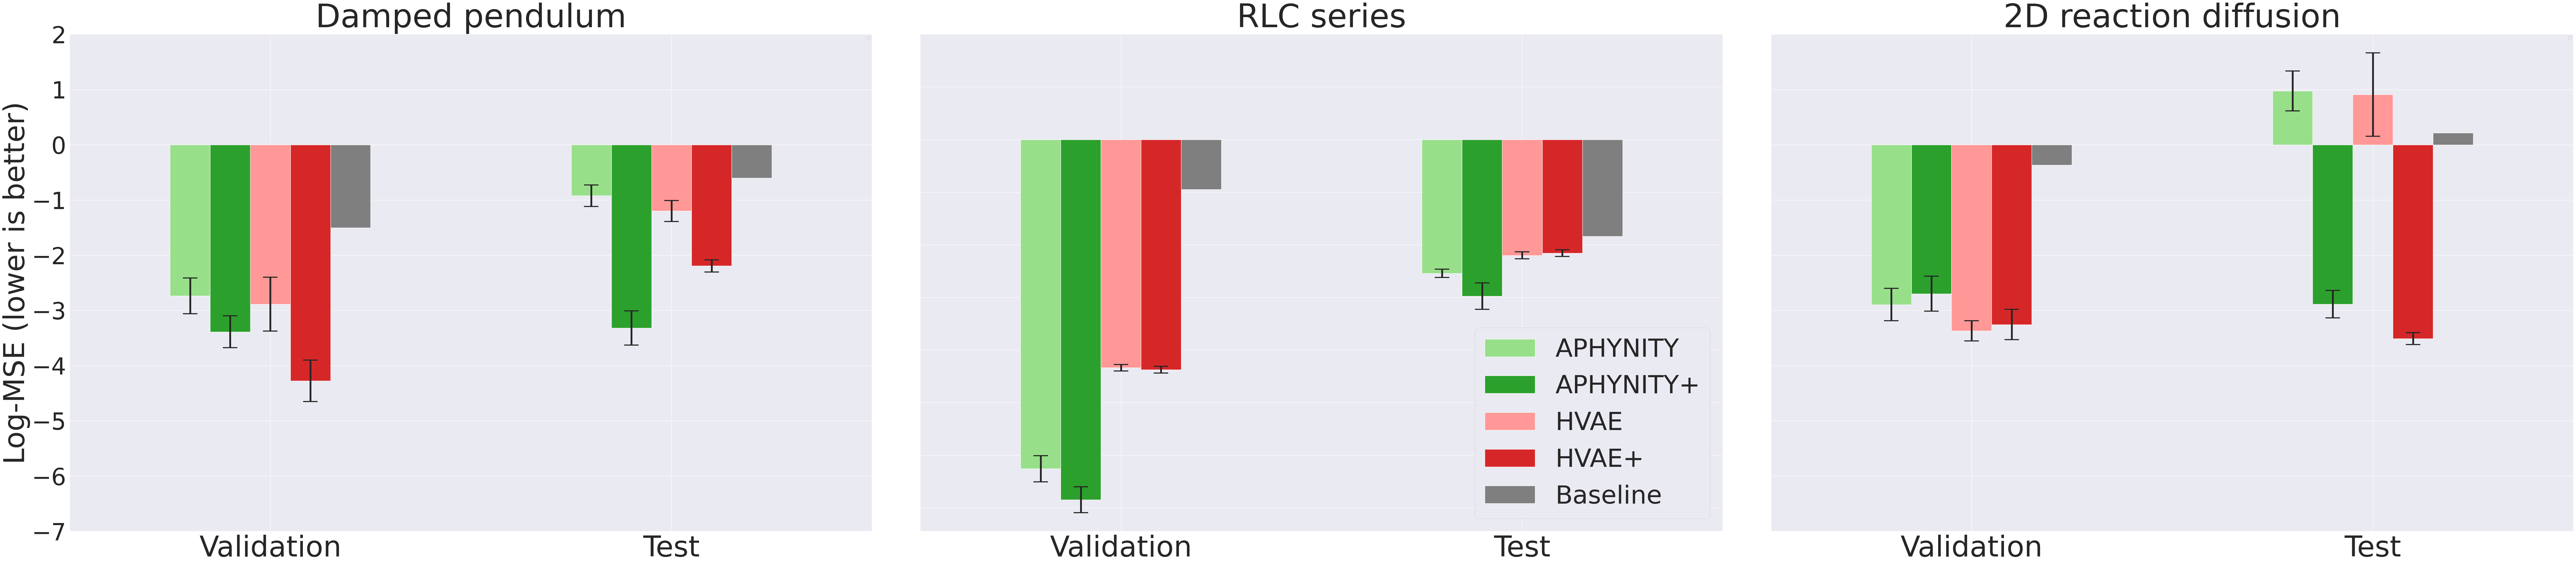
\includegraphics[width=.98\textwidth]{figures/results_log_mse.png}
    \vspace{-1em}
    \caption{The average log-MSEs over 10 runs for three synthetic problems on the validation and test sets. We compare HVAE (in red) and APHYNITY (in green), in light colours, to their expert augmented versions HVAE+ and APHYNITY+, in darker colours. \textit{On the test sets, AHMs outperform the original models, and by a large margin on the pendulum and diffusion problems. Moreover, augmentation conserves the relatively good performance on the validation set (IID w.r.t. the training set).}}
    \label{fig:log_mse}
    \vspace{-1.em}
\end{figure*}

\subsection{Problem description} \label{sec:problems_description}
We assess the benefits of expert augmentation on three controlled problems described and simulated by the ODE
\begin{align}
    \frac{dy_t}{dt} = F_e(y_t; z_e) + F_a(y_t; z_a), \label{eq:generic_ode}
\end{align}
where $F_e: \mathcal{Y}_t \times \mathcal{Z}_e \rightarrow \mathcal{Y}_t$ is the expert model and $F_a: \mathcal{Y}_t \times \mathcal{Z}_a \rightarrow \mathcal{Y}_t$ complements it. In our notation $X$ is the initial state $y_0$ and the response $Y$ is the sequence of states $y_{1:t_1}:=[y_{i\Delta t}]_{i=1}^{t_1 \!/\! \Delta t}$. For all experiments we train the models to maximize $p_{\theta, \psi}(y=y_{1:t_1}|x=y_0)$ on the training data. We validate and test the models on the predictive distribution $p(y=y_{1:t_2}|x=y_0, x_o=y_0, y_o=y_{1:t_1})$, where $t_2 > t_1$ assesses the generalization over time. A brief description of the different problems is provided below.

\textbf{The damped pendulum} is often used as an example in the hybrid modelling literature \citep{APHYNITY, HVAE}. The system's state at time $t$ is $y_t = \begin{bmatrix}\theta_t & \dot \theta_t\end{bmatrix}^T$, where $\theta_t$ is the angle of the pendulum at time t and $\dot \theta_t$ its angular speed. The evolution of the state over time is described by \eqref{eq:generic_ode}, where $z_e:=\omega$, $z_a=\alpha$ and
\begin{align}
    F_e := \begin{bmatrix}\dot \theta &  -\omega_0^2 \sin \theta   \end{bmatrix}^T \quad \text{and} \quad F_a := \begin{bmatrix}0 &  -\alpha \dot \theta \end{bmatrix}^T.
\end{align}
The corresponding systems are defined by the damping factor $\alpha$ and $\omega_0$, the fundamental frequency of the pendulum.

\textbf{The RLC series circuits} are electrical circuits made of 3 electrical components that may model a large range of transfer functions. These models are often used in biology (e.g., the Hodgkin-Huxley class of models~\citep{hh-model}, in photoplethysmography~\citep{ppg-model}) and in electrical engineering to model the dynamics of various systems. The system's state at time $t$ is $y_t = \begin{bmatrix}U_t & I_t\end{bmatrix}^T$, where $U_t$ is the voltage around the capacitance and $I_t$ the current in the circuit. The evolution of the state over time is described by \eqref{eq:generic_ode}, where $z_e:=\{L, C\}$, $z_a= \{R\}$ and

\begin{align}
    F_e := \begin{bmatrix}\frac{I_t}{C} \\ \frac{1}{L} (V(t) - U_t) \end{bmatrix} \quad \text{and} \quad F_a := \begin{bmatrix}0 \\- \frac{R}{C}I_t\end{bmatrix}.
\end{align} The dynamics described by the RLC circuit is more diverse than for the pendulum and the system can be hard to identify. This system is characterised by the resistance $R$, capacitance $C$, and inductance $L$, provided $V(t)$ is known.

\textbf{The 2D reaction diffusion} was used by \citet{APHYNITY} to assess the quality of APHYNITY. It is a 2D FitzHugh-Nagumo on a $32 \times 32$ grid. The system's state at time $t$ is a $2\times 32 \times 32$ tensor $y_t = \begin{bmatrix}u_t & v_t\end{bmatrix}^T$. The evolution of the state over time is described by \eqref{eq:generic_ode}, where $z_e:=\{a, b\}$, $z_a= \{k\}$ and 
\begin{align}
    F_e := \begin{bmatrix}a \Delta u_t \\ b \Delta v_t \end{bmatrix} \quad \text{and} \quad F_a := \begin{bmatrix}R_u(u_t, v_t;k) \\R_v(u_t, v_t)\end{bmatrix},
\end{align}
where $\Delta$ is the Laplace operator, the local reaction terms are $R_u(u, v;k) = u - u^3 - k -v$ and $R_v(u, v) = u - v$.
This model is interesting to study as it considers a state space for which neural architectures may have a real advantage compared to other ML models.


In the following experiments we analyze the effect of our data augmentation strategy on APHYNITY and HVAE. All models explicitly use the assumption that the interaction model follows the structure of \eqref{eq:generic_ode}. For each problem the validation and test sets are respectively IID and OOD with respect to the training distribution. The best models are always selected based on validation performance, that is with samples from $\Omega$. We provide additional details on the different expert models, dataset creation, and neural networks architectures in \appref{app:exp_details}.

\subsection{Results}
\paragraph{Performance gain from augmentation.}
\textit{This experiment demonstrates that HVAE and APHYNITY are not robust to OOD test scenarios in opposition to the corresponding AHMs, as shown in \figref{fig:diffusion_shift}} for the 2D diffusion problem and in \appref{app:supp_results} for the two other problems. We emphasize that our intention is not to declare a winner between HVAE and APHYNITY. Indeed, both algorithms have already demonstrated superior performance than black box ML models. Hence, we only report a very simple baseline that is the mean value of the signals. We want to compare performance in OOD settings and empirically validate the benefit of AHMs.
We compare the predictive performance in \figref{fig:log_mse} (see \Cref{tab:synth_log_mse} for the raw numbers).  Although classical hybrid learning strategies do very well on the IID validation set, they exhibit poor generalization on OOD test sets for all three problems. We also observe some disparity between APHYNITY and HVAE. In addition to different learning strategies, this is probably due to differences in the networks' architectures as they were respectively inspired from the corresponding pendulum experiment in each paper. However, even if one method may outperform the other for some problems, they both benefit from our augmentation strategy (APHYNITY+, HVAE+). Overall, the effect of augmentation goes up to dividing the test error by a factor of $e^{4.6}\approx 100$ in some cases. 

\begin{table}[]
    \small
    \centering
    \setlength{\tabcolsep}{4pt}
    \begin{tabular}{c c|c c | c c}
        Dataset & & APH. & HVAE & APH.+ & HVAE+ \\ \hline
%        & Train & &  &  &  &  \\
       \multirow{2}{*}{Pendulum} & Valid. & $6_{\pm 2}$ & $3_{\pm 1}$ & $6_{\pm 2}$ & $2_{\pm 1}$ \\
        & Test & $66_{\pm 9}$ & $117_{\pm 10}$ & $10_{\pm 4}$ & $11_{\pm 2}$    \\ \hline
%        & Train & &  &  &  &  \\
       \multirow{2}{*}{RLC} & Valid. & $6_{\pm 3}$ & $38_{\pm 2}$ & $7_{\pm 5}$ & $28_{\pm 1}$ \\
        & Test & $17_{\pm 3}$ & $25_{\pm 2}$ & $5_{\pm 2}$ & $12_{\pm 1}$ \\ \hline
        
       \multirow{2}{*}{Diffusion} & Valid. & $2_{\pm 0}$ & $2_{\pm 0}$ & $2_{\pm 0}$ & $2_{\pm 0}$ \\
        & Test & $27_{\pm 2}$ & $32_{\pm 10}$ & $3_{\pm 1}$ & $2_{\pm 0}$\\ \hline
    \end{tabular}
    \caption{Comparison of mean relative precision (in $\%$, $\pm$ indicates one standard deviation) over 10 runs of predicted physical parameters of different hybrid modelling strategies in validation and OOD test settings. Augmented versions are denoted with a $+$. \textit{While the accuracy of APHYNITY and HVAE is good on the validation set, it collapses on the OOD test set. On the opposite, the augmented versions perform well on both validation and test sets.}}
    \label{tab:param_acc}
    \vspace{-1.5em}
\end{table}

\paragraph{Stability for non-exact models.}
The empirical results from \figref{fig:log_mse} are very important as they show that even when the decoder is not $\Omega\textit{-exact}$ (and hence not $\accentset{+}{\Omega}\textit{-exact}$), augmentation is still useful. In particular, \Cref{tab:param_acc} shows that the encoder does not predict the physical parameters perfectly. This indicates that the encoder is not $\Omega\textit{-exact}$ and neither should be the decoder. This table shows the relative error on the physical parameters computed as $\sum_{i=1}^k\frac{1}{k}\left|\frac{z_e^i - \mu_\theta^i}{z_e^i}\right|$, where $\mu_\theta^i$ is the estimated most likely value of the $i^{th}$ component of the physical parameters. We first notice that APHYNITY and HVAE perform differently and their performance depends on the specific problem. While APHYNITY accurately estimates the physical parameters on the IID validation set for the 3 problems, HVAE's performance are mixed on the RLC problem as it makes prediction that are $38\%$ away from the nominal parameter value on average whereas APHYNITY reduces this error to $6\%$. Interestingly, we observe that the proposed augmentation strategies improve the encoder such that it accurately estimates the physical parameters also on the OOD test set even for HVAE on the RLC problem. This confirms that the augmentation strategy is helpful even when the hybrid model is not $\Omega\textit{-exact}$. As a conclusion, augmented hybrid learning outperforms classical hybrid learning both on the predictive accuracy and at inferring the expert variables.

\paragraph{Effect of out of expertise shift.}
\textit{This experiment shows that our augmentation strategy may remain beneficial even when the train and test supports of $z_a$ are not identical.} This scenario corresponds to samples $(x, y)$ generated by $(z_a, z_e) \in (\accentset{\ast}{\mathcal{Z}}_a \setminus \mathcal{Z}_a) \times \tilde{\mathcal{Z}}_e$ depicted by the violet domains in \figref{fig:ood_vizu}. In \figref{fig:za_shifted} we observe the log-MSE of augmented and non-augmented hybrid models trained for $(z_a, z_e) \in \mathcal{Z}_a \times \mathcal{Z}_e$ on test data that are generated with $(z_a, z_e) \in \tilde{\mathcal{Z}}_a \times \tilde{\mathcal{Z}}_e$. For the pendulum, the support over $z_a=\alpha$ is $\left[0, 0.3\right]$ in train and $\left[0.3, 0.6\right]$ in test; For the 2D reaction diffusion, $z_a=k$ is $\left[0.003, 0.005\right]$ in train and $\left[0.005, 0.008\right]$ in test. We observe that augmented models outperform the original models by a large margin. These results suggest that augmentation could be very valuable in practice, even when the distribution shift is also caused by non expert variables. However, if the shift on $z_a$ becomes the dominant effect, augmented models also eventually becomes vulnerable to shifts on $z_e$ as demonstrated by supplementary experiments in \appref{app:exp_details}.  

\begin{figure}
    \centering
    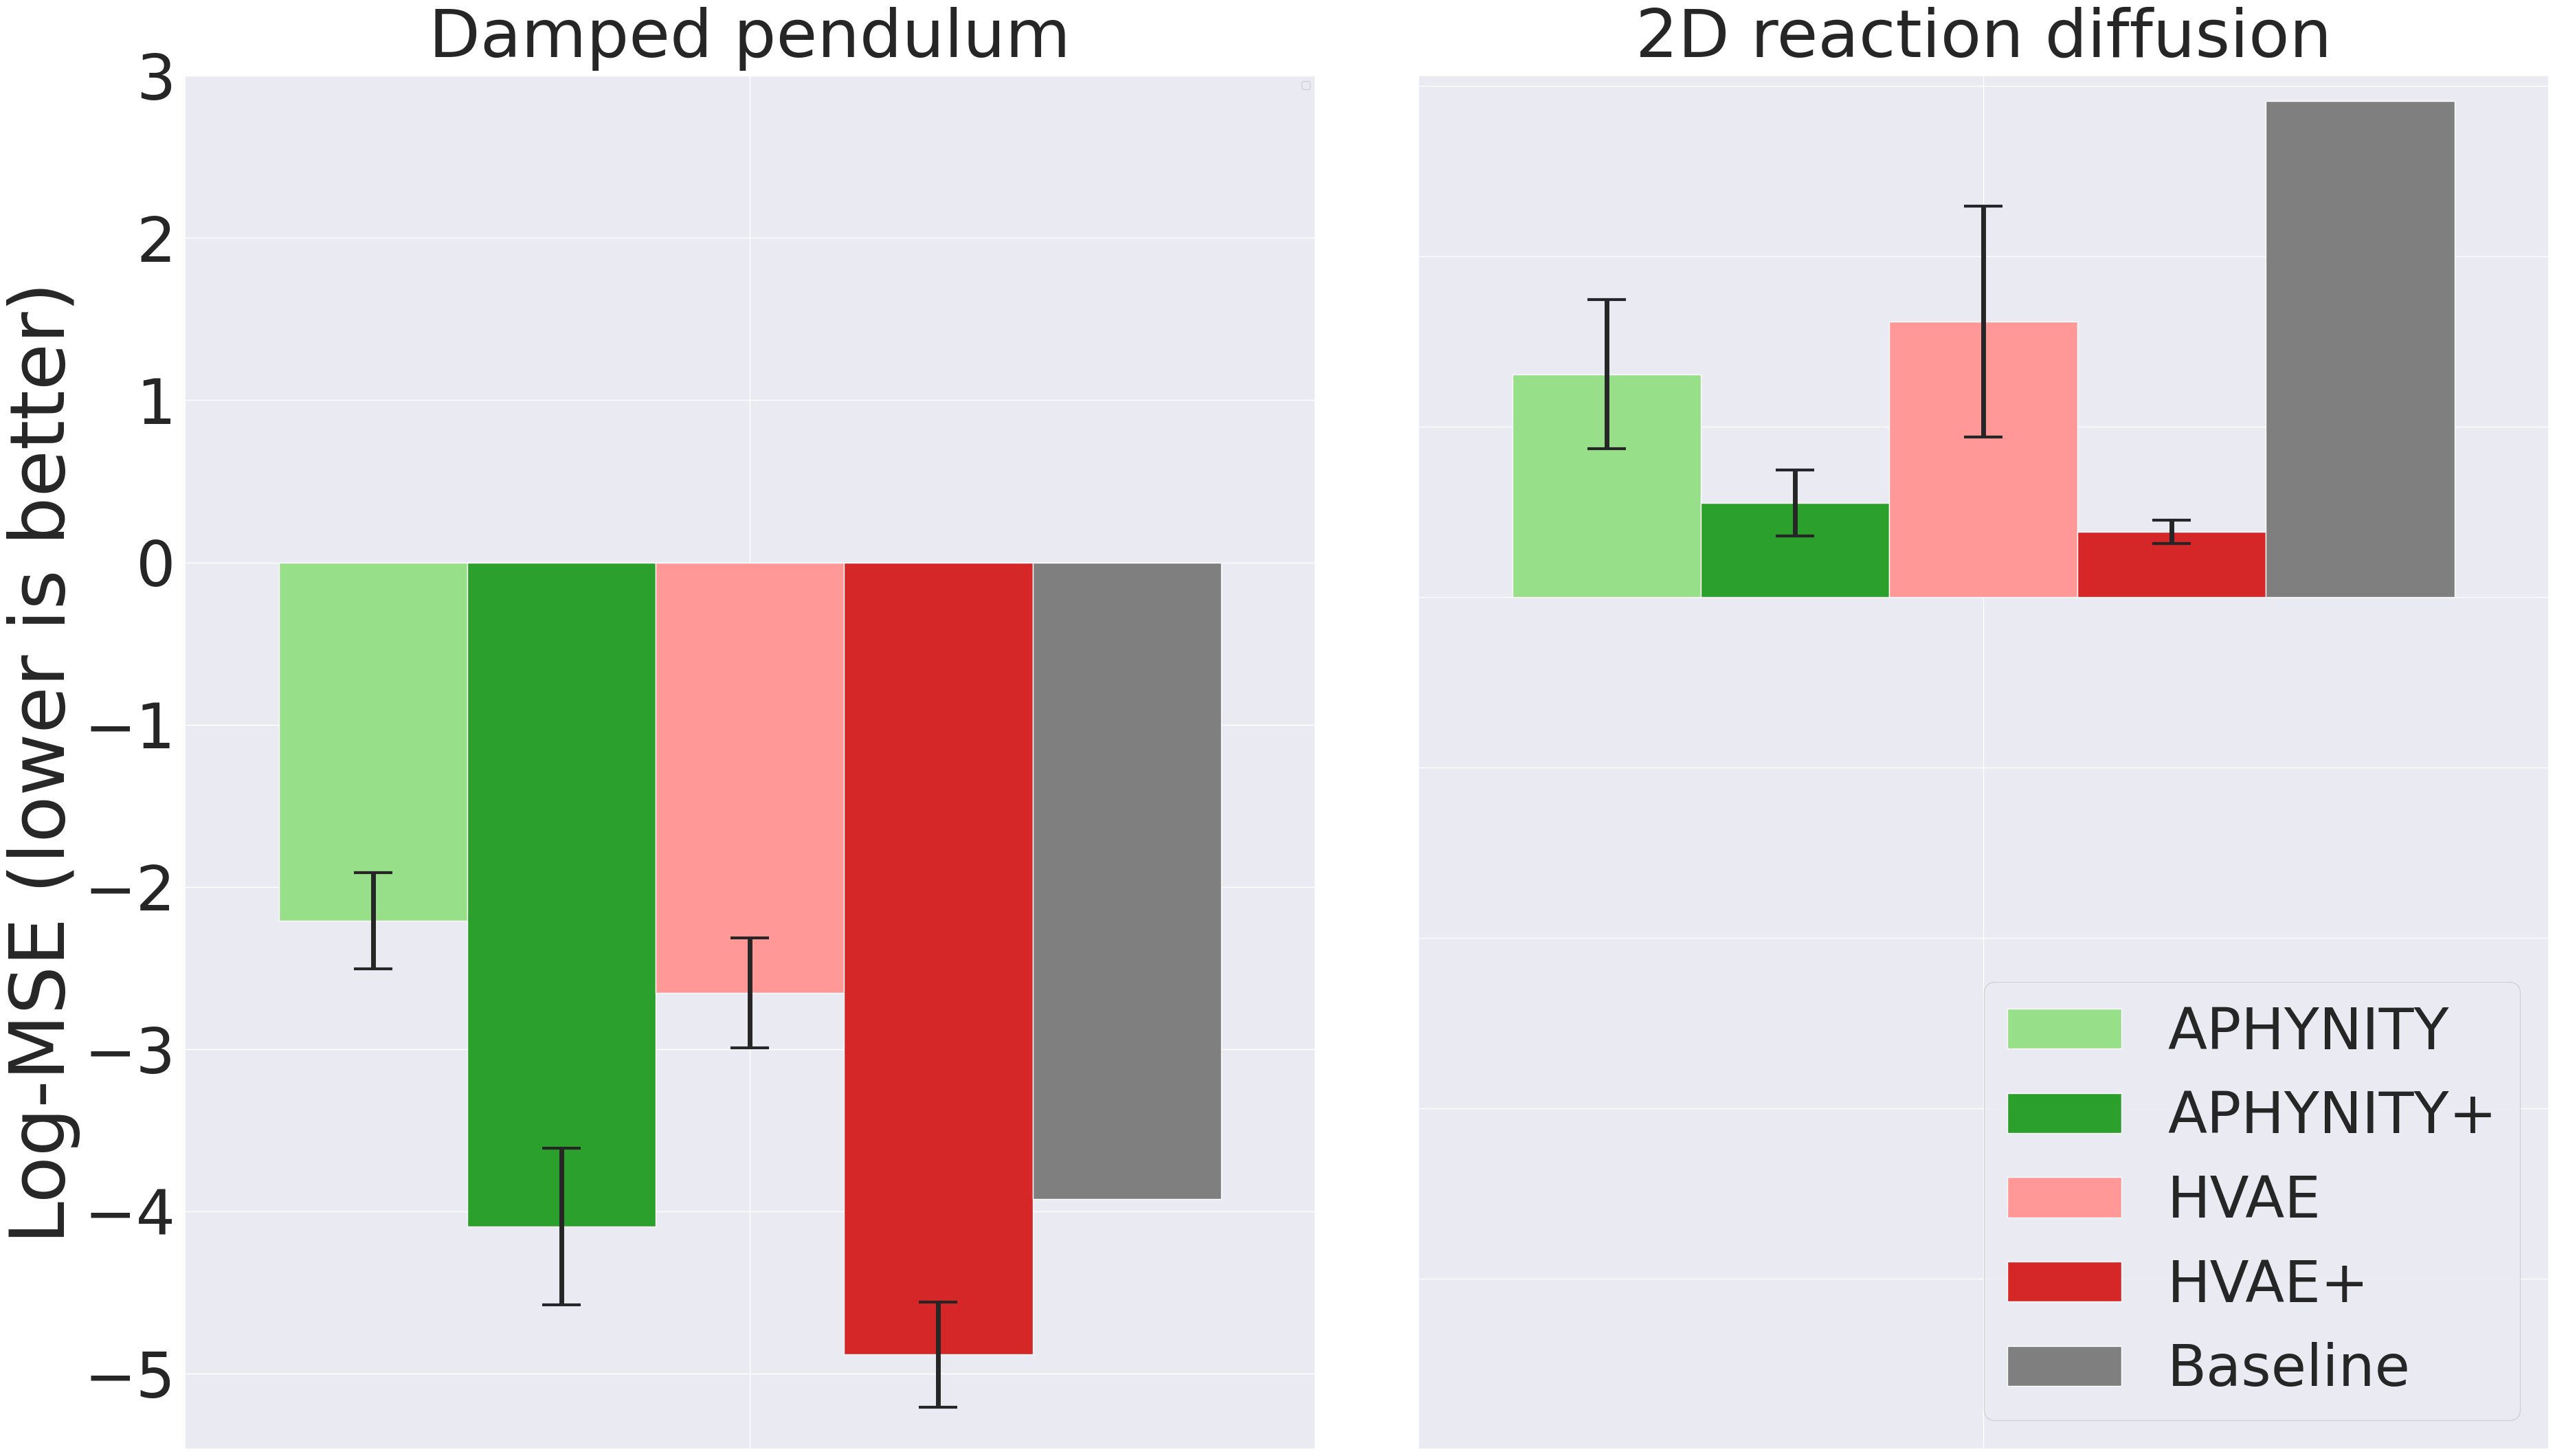
\includegraphics[width=.48\textwidth]{figures/results_log_mse_za_OOD-4.png}
    \vspace{-2em}
    \caption{The average log-MSEs over 10 runs for the \textit{damped pendulum} and \textit{2D reaction diffusion} problems on a test distribution for which $z_a$, in addition to $z_e$, is also shifted. \textit{AHM achieves better peformance than stand HyL algorithms even when the test distribution support $z_a$ differs from the training.}}
    \label{fig:za_shifted}
    \vspace{-1.em}
\end{figure}

%%%%%%%%%%%%%%%%%%%%%%%%%%%%%%%%%% 5 Related work %%%%%%%%%%%%%%%%%%%%%%%%%%%%%%%%%%
\section{Related work}
\subsection{Hybrid modelling}
Hybrid Learning (HyL), or gray box modelling as called in its early days in the 90's \citep{old_hl_1, old_hl_2, old_hl_3, old_hl_4, old_hl_5}, has been an appropriate method to learn models that are both expressive and interpretable, while also allowing them to be learnt on fewer data. The interest for HyL \citep{hl_1, hl_2, hl_3, hl_4, hl_5, hl_6, metnet2} has greatly renewed since the outbreak of recent neural network architectures that simplify the combination of physical equations within ML models. As an example, Neural ODE~\citep{NODE} and convolutional neural networks~\citep[][CNN]{lecun_cnn} are privileged architectures to work with dynamical systems described by ODEs or PDEs. While most of the HyL's literature focus on the predictive performance of hybrid models, recent work have also showed that HyL may help to infer the physical parameter accurately \citep{APHYNITY, HVAE}. This is aligned with \citet{nuisance_para} (see Section 40.2.2.2) which observe that inference on incomplete models results in a \textit{systematic bias}. Similar to HyL, they extend the model with \textit{nuisance} parameters in order to improve its fidelity, and to reduce the systematic bias.

In this work, we decided to study \citet{APHYNITY} and \citet{HVAE} for two reasons that distinguish them from the rest of the HyL literature. First, these are notable examples of HyL algorithms that can be applied to a broad class of problems in contrast to papers that focus on specific applications \citep{hl_2,hl_3}. Second, those methods also learn a reliable inference model for the physical parameters, suggesting that the expert model is used properly in the generative model, which is a key assumption for our augmentation. While \citet{HVAE} claim to achieve robustness with HyL, we argue that this statement is incomplete as HVAE fails in OOD settings. In particular, their approach is only able to generalize with respect to unseen time or initial state if the model correctly identifies the latent variables $z_a, z_e$. 

\subsection{Combining hybrid modelling and data augmentation}
Close to our idea is the one proposed in \citet{gan_hl} where they train a GAN model that improves the realism of a simulated image while conserving its semantic content (e.g. eyes colour) as modeled by the simulation parameters. The generated data with their annotations may then be used for a downstream task, such as inferring the properties of real images that corresponds to simulation parameters. The GAN objective from \citet{gan_hl} requires that the two distributions induced by the semantic content of real and simulated data are identical. On the opposite, we consider training data that corresponds to expert parameters with limited diversity, and overcome this scarcity with expert augmentation. Another line of work similar to ours is Sim2Real, which considers the task of transferring a model trained on simulated data to real world \citep{sim2real-1, sim2real-2, sim2real-3}. Robust HyL, as a way to enhance simulations, could be used for Sim2Real.

%\subsection{Robust ML}
\subsection{Robust ML and Invariant Learning}
Various statistical methods have been introduced to ensure models generalize under distribution shift. Domain-adversarial objectives aimed at learning (conditionally) invariant predictors \citep{ganin2016domain,zhang2017aspect,li2018deep}, GroupDRO \citep{groupDRO_ICLR} optimizing for worst-case loss over multiple domains and IRM~\citep{IRM} as well as sub-group calibration \citep{wald2021calibration} aiming to satisfy calibration or sufficiency constraints to learn features invariant across domains. Extensions, able to infer domain labels from training data have been proposed as well \citep{lahoti2020fairness,creager2021environment}, partially inspired by fairness objectives \citep{hebert2018multicalibration,kim2019multiaccuracy}. In contrast to AHM, all of these methods rely on the variation of interest being present in the training data.

%%%%%%%%%%%%%%%%%%%%%%%%%%%%%%%%%% 6 Discussion %%%%%%%%%%%%%%%%%%%%%%%%%%%%%%%%%%
\section{Discussion}
We now examine the assumptions we made to derive our augmentation strategy and discuss potential limitations.
\paragraph{Erroneous interaction model.}
The exactness of the hybrid component $p_\theta(y|x, y_e, z_a)$ is a critical assumption underlying our expert-based augmentation strategy. Unfortunately, this component is learned from training data only, hence we cannot prove its exactness on the test domain, which corresponds to a different domain $\mathcal{Y}_e$. However, we argue that soft assumptions on the class of interaction model may alleviate this problem. As an example, when we consider an additive hybrid model, as in APHYNITY~\citep{APHYNITY}, and embed this hypothesis into the interaction model, generalization to unseen $y_e$ follows. When this assumption is too strong, we could still expect generalization of $p_\theta(y|x, y_e, z_a)$ because HyL drives $y$ samples from $p_\theta$ to be close to $y_e$. It implies that the corresponding function approximator is smooth, which helps generalization to unseen scenarios. This contrasts with the encoder $q_\psi$ for which a a good inductive bias usually is not available. 
\paragraph{Diagnostic.}
While crucial, we cannot guarantee the exactness of the decoder $p_\theta$ in general because we only evaluate the encoder and the decoder jointly on data points $(x, y, x_o, y_o)$. However, in some cases we can detect model misspecification by observing that the predictive model $p_{\theta, \psi}(y|x, x_o, y_o)$ is imperfect. Making this observation is not always simple as it requires prior knowledge on the expected accuracy of an exact model. However, when the system is deterministically identifiable, we may argue that the accuracy should be only limited by the intrinsic noise between $x$ and $y$ given $z_a$ and $z_e$.

\paragraph{Relaxing exactness.}
Even with a strong inductive bias on the decoder, achieving exactness is hopeless in practical settings. However, our experiments demonstrate that expert-augmentation works in practice. We can explain this by taking a look at \figref{fig:ood_vizu}. If the generative model that maps $x$ and $(z_a, z_e)$ is incorrect, the mapping from $\mathcal{Z}_a$ and $\mathcal{Z}_e$ could be slightly off from $\accentset{+}{\Omega}$.  However, this does not preclude the set of augmented samples to be closer to $\accentset{+}{\Omega}$ than $\Omega$ and to induce a better predictive model on $\accentset{+}{\Omega}$ than the original model trained only on $\Omega$.

\paragraph{Limitations}
We considered expert models that are parameterized by a small number of parameters, which can be covered densely via sampling. Covering densely a higher dimensional parameter space with the augmentation strategy becomes quickly impossible, hence a smarter sampling strategy would be required, such as worst-case sampling. Another difficulty is to choose a plausible range of parameters that contains both the train and the test support, this will often require a human expert in the loop. Finally, we assume that the train distribution of $z_a$ should be representative of the test distribution, we empirically observed that a softer version of this assumption could be enough. However, performance will eventually decline as the support of the test distribution for $z_a$ is far from the training domain.

%%%%%%%%%%%%%%%%%%%%%%%%%%%%%%%%%% 7 Conclusion %%%%%%%%%%%%%%%%%%%%%%%%%%%%%%%%%%
\section{Conclusion}
In this work, we describe HyL with a probabilistic model in which one component of the latent process, denoted the expert model, is known. In this context, we establish that state-of-the-art HyL algorithms are vulnerable to distribution shifts even when the expert model is well defined for such configurations. Grounded in this formalisation, we derive that expert augmentations induce robustness to OOD settings. We discuss how our assumptions can transfer to real-world settings and describe how to diagnose potential shortcomings. Finally, empirical evidence asserts that expert augmentations may be beneficial even when one of our assumptions on the class of distribution shift is violated.

Our augmentation is applicable to a large class of hybrid models, hence it should benefit from future progress in HyL. Thus, we believe research in HyL and formally defining its targeted objectives is an important direction for further improving the robustness of hybrid models. As an example, the minimal description length principle \citep{mdl_book} could be a great resource to investigate the balance between the model's capacity and robustness. Finally, robust ML models must eventually translate to real-world applications, hence a next step would be to apply AHMs to real-wold data. Paving the way to future research combining AHM with robust ML methods. 

%%%%%%%%%%%%%%%%%%%%%%%%%%%%%%%%%% Acknowledgements %%%%%%%%%%%%%%%%%%%%%%%%%%%%%%%%%%
\section*{Acknowledgements}
We would like to acknowledge Andy Miller, Dan Busbridge, Jason Ramapuram, Joe Futoma, and Mark Goldstein for providing useful feedback on this manuscript or an earlier version of it. 

\bibliography{main}
\bibliographystyle{icml2022}


\clearpage
\onecolumn
\appendix
\section{Additional description of expert augmentation}\label{app:ahm_desc}
We provide the procedure to do expert augmentation for robust HyL as the sequence of steps below.
\begin{enumerate}
    \item Train both the encoder $q_\psi(z_a, z_e|x, y)$ and the interaction model $p_\theta(y|x_o, z_a, y_e)$ with a HyL algorithm, by minimizing the corresponding loss $\mathcal{L}(\psi, \theta) = \mathbb{E}_{\mathcal{D}}\left[\ell(x, y; \theta, \psi)\right]$ on the training set $\mathcal{D}$;
    \item Decide on an augmented distribution $\accentset{+}{p(z_e)}$ for $z_e$ that contains both train and test scenarios;
    \item Reproduce the following steps to generate a dataset $\accentset{+}{\mathcal{D}}$ of observations and expert variables $(x, y, z_e) \sim \mathbb{E}_{p(z_a)p(y_e|z_e, x, y)}\left[ p(z_e) p(x) p_\theta(y|y_e, z_a, x)\right]$:
    \begin{enumerate}
        \item Sample $(x_o, y_o)$ from the data;
        \item Sample $z_a$ from the posterior $q_\psi(z_a|x_o, y_o)$;
        \item Sample $z_e$ from $\accentset{+}{p(z_e)}$;
        \item Push forward $x, z_a$ and $z_e$ in the generative model as $y_e \sim p(y_e|x_o, z_e)$ and $y \sim p_\theta(y|x_o, z_a, y_e)$;
        \item Add the triplet $(x_o, y, z_e)$ to the augmented training set $\accentset{+}{\mathcal{D}}$.
    \end{enumerate}
    \item Freeze the interaction model, and fine-tune the encoder $q_\psi(z_a, z_e|x, y)$ on the augmented dataset $\accentset{+}{\mathcal{D}}$ by minimizing $\accentset{+}{\mathcal{L}}(\psi, \theta) = \mathbb{E}_{\accentset{+}{\mathcal{D}}}\left[\ell(x, y; \theta, \psi) - \log q_\psi(z_e|x, y)\right]$.
\end{enumerate}
\section{Additional details on experiments}\label{app:exp_details}
\subsection{Damped pendulum}
\paragraph{Datasets.}
We use Neural Ordinary Differential Equations (NODE) \citep{NODE} to solve the ODE ruling the damped pendulum. Each sample is simulated for $t_0=0s$, $t_1=5s$, and $t_2=20s$, with a time resolution equal to $0.1$ second. The models are trained with only the realizations between $t_0$ and $t_1$. At test and validation time, the pair $(x_o, y_o) = (y_0, [y_{i\Delta t}]_{i=1}^{t_1 \!/\! \Delta t})$, $x=y_{t_1}$ and the model predicts $y=[y_{i\Delta t}]_{i=t_2 \!/\! \Delta t + 1}^{t_2 \!/\! \Delta t}$. The initial angular speed is always $0$ and $\theta_0 \sim \mathcal{U}(-\frac{\pi}{2}, \frac{\pi}{2})$.

The training set is made of $1000$ samples and the validation set of 100 samples. They are both generated by sampling uniformly $z_a := \alpha$ from $\mathcal{Z}_a := \left[ 0, 0.6 \right]$ and $z_e := \omega_0$ from $\mathcal{Z}_e := \left[ 1.5, 3.1 \right]$. The shifted test set contains 100 samples generated by sampling uniformly $z_a$ in $\mathcal{Z}_a$ and $z_e$ in $\tilde{\mathcal{Z}}_e := \left[0.5, 1.5 \right]$.
\paragraph{APHYNITY.}
Our model is composed of a $1$-layer RNN with $128$ units that encodes the input signal $y_{0:t_1}$ as $h(y_{0:t_1}) \in \mathbb{R}^{128}$. An MLP with $3$ layers of $150$ units and ReLU activations maps $h$ to $\mathbb{R}_+$ to predict $\omega_0$. The function $f_a: \mathbb{R}^{128} \times \mathbb{R}^2$ is an MLP with $3$ layers of $50$ units and ReLU activations (no activation for the last layer). The models are trained for $50$ epochs with Adam with no weight decay and a learning rate equal to $0.0005$. For the Lagrangian optimization we use $N_{iter}=5, \lambda_0=10, \tau_2 = 5$ (see \citep{APHYNITY}. The augmented data are generated by sampling uniformly $z_e \in \accentset{+}{\mathcal{Z}}_e := \left[0.5, 3.5\right]$ and $z_a$ from the marginal predictive prediction of the model, that is we use the training dataset to infer values of $z_a$ and use these as samples. The batch size is $100$.

\paragraph{HVAE.}
We use the notations from \citet{HVAE} to describe the architecture of the VAE. The network $g_{p, 1}: \mathbb{R}^2 \times \mathbb{R}^{d_a}$, where $d_a=1$ is the size of the latent space for the interaction model, is supposed to filter the observations so that they can be generated by the expert model. It has $2$ hidden layers with $128$ units, $g_{p, 2}$ is an MLP with the following hidden layers $\left[128, 128, 256, 64, 32\right]$ and takes the full sequence of filtered states and predicts the mean and variance of a normal distribution that parameterize the posterior $p_\theta(z_e|x, y, z_a)$. Another network, $g_a$ takes the sequence of observations and predict the posterior distribution of $z_a$ as a normal distribution. This network has the following hidden layers $\left[256, 256, 128, 32\right]$. All networks have SeLU activations. In general the decoder of HVAE can be anything that combines the expert model in order to produce samples in the observation space, as we made the hypothesis that the ODE is just missing an additive term, the decoder is a NODE where the function is the sum of $f_e$ and $f_a$ a two hidden layers MLP with $64$ units and SeLU activation (except for the last layer that has no activation). The likelihood model is also Gaussian with the mean being predicted by the NODE and the variance learned but shared for all observations. For additional details on our architecture and implementation details we encourage the interested reader to check our code. 

The networks are trained jointly for $1000$ epochs with Adam optimizer, with a learning rate equal to $0.0005$, weight decay equal to $0.000001$ and batch size $200$. The other parameters are set to $\gamma = 1$, $\alpha=0.01$ and $\beta=0.01$. The HVAE also relies on some augmentation during training and in order to compare fairly our model to theirs we use the same distribution for our augmentation and theirs that is $z_a \sim \mathcal{N}(0, I)$ and $z_e \sim \mathcal{U}(0.5, 3.5)$. 

\subsection{RLC series}
\paragraph{Datasets.}
Similar to the damped pendulum, we use NODE to solve the ODE ruling the RLC circuit. Each sample is simulated for $t_0=0s$, $t_1=5s$, and $t_2=20s$, with a time resolution equal to $0.1$ second. The models are trained with only the realizations between $t_0$ and $t_1$. At test and validation time, the pair $(x_o, y_o) = (y_0, [y_{i\Delta t}]_{i=1}^{t_1 \!/\! \Delta t})$, $x=y_{t_1}$ and the model predicts $y=[y_{i\Delta t}]_{i=t_2 \!/\! \Delta t + 1}^{t_2 \!/\! \Delta t}$. In all experiments, the initial value for $U_0 \sim \mathcal{N}(0, 1)$ and $I_0=0$, the voltage source delivers a AC + DC tension $V(t) = 2.5 \sin(4 \pi t) + 1$.

The training set is made of $2000$ samples and the validation set of 100 samples. They are both generated by sampling uniformly $z_a := R$ from $\mathcal{Z}_a := \left[ 1, 3 \right]$ and $z_e := \left[L, C\right]$ from $\mathcal{Z}_e := \left[ 1, 3 \right] \times \left[ 0.5, 1.5 \right]$. The shifted test set contains 100 samples and is generated by sampling uniformly $z_a$ in $\mathcal{Z}_a$ and $z_e$ in $\tilde{\mathcal{Z}}_e := \left[ 3, 5 \right] \times \left[ 1., 2.5 \right]$.
\paragraph{APHYNITY.}
Our model is composed of a 1-layer RNN with 128 units that encodes the input signal $y_{0:t_1}$ as $h(y_{0:t_1}) \in \mathbb{R}^{128}$. An MLP with $3$ layers of $200$ units and ReLU activations maps $h$ to $\mathbb{R}_+^2$ that predicts $L$ and $C$. The function $f_a: \mathbb{R}^{128} \times \mathbb{R}^2$ is an MLP with $3$ layers of $150$ units and ReLU activations (no activation for the last layer). The models are trained for $50$ epochs with Adam with no weight decay and a learning rate equal to $0.0005$. For the Lagrangian optimization we use $N_{iter}=5, \lambda_0=10, \tau_2 = 5$ (see \citep{APHYNITY}). The augmented data are generated by sampling uniformly $z_e \in \accentset{+}{\mathcal{Z}}_e := \left[1, 5\right] \times \left[0.5, 2.5\right]$ and $z_a$ from the marginal predictive prediction of the model, that is we use the training dataset to infer values of $z_a$ and use these as samples. The batch size is $100$.

\paragraph{HVAE.}
We use the same networks' architectures than for the damped pendulum experiment. Except that $g_{p, 1}$ is has $3$ hidden layers with $100$ units.

The networks are trained jointly for $1000$ epochs with Adam optimizer, with a learning rate equal to $0.0005$, weight decay equal to $0.000001$ and batch size $100$. The other parameters are set to $\gamma = 1$, $\alpha=0.01$ and $\beta=0.01$. The HVAE also relies on some augmentation during training and in order to compare fairly our model to theirs we use the same distribution for our augmentation and theirs that is $z_a \sim \mathcal{N}(0, I)$ and $z_e \sim \mathcal{U}(1, 5) \times \mathcal{U}(0.5, 2.5)$. 

\subsection{2D reaction diffusion}
\paragraph{Datasets.}
Similar to the damped pendulum, we use NODE to solve the PDE ruling the reaction diffusion. We closely follow the experimental setting described in \citet{APHYNITY} and approximate the Laplace operator with a $3 \times 3$ discrete version of the operator. Each sample is simulated for $t_0=0s$, $t_1=1s$, and $t_2=5s$, with a time resolution equal to $0.1$ second. The models are trained with only the realizations between $t_0$ and $t_1$. At test and validation time, the pair $(x_o, y_o) = (y_0, [y_{i\Delta t}]_{i=1}^{t_1 \!/\! \Delta t})$, $x=y_{t_1}$ and the model predicts $y=[y_{i\Delta t}]_{i=t_2 \!/\! \Delta t + 1}^{t_2 \!/\! \Delta t}$. The initial state is sampled from a uniform distribution in $\left[0, 1\right]$.

The training set is made of 2000 samples and the validation set of 100 samples. They are both generated by sampling uniformly $z_a := k$ from $\mathcal{Z}_a := \left[ 0.003, 0.005 \right]$ and $z_e := \left[a, b\right]$ from $\mathcal{Z}_e := \left[ 0.001, 0.002 \right] \times \left[ 0.003, 0.007 \right]$. The shifted test set contains 100 samples and is generated by sampling uniformly $z_a$ in $\mathcal{Z}_a$ and $z_e$ in $\tilde{\mathcal{Z}}_e := \left[ 0.002, 0.004 \right] \times \left[ 0.001, 0.1 \right]$.
\paragraph{APHYNITY.}
Our model is composed of a deep CNN that encodes the input sequence of 10 images. The exact architecture can be found in the code. The dimension of $z_a$ is equal to 10. Similarly to \citet{APHYNITY} the function $f_a$ is a 3-layers CNN with ReLU activations. The models are trained for $500$ epochs with Adam with no weight decay and a learning rate equal to $0.0005$. For the Lagrangian optimization we use $N_{iter}=1, \lambda_0=10, \tau_2 = 5.$. The augmented data are generated by sampling uniformly $z_e \in \accentset{+}{\mathcal{Z}}_e := \left[0.001, 0.004\right] \times \left[0.001, 0.01\right]$ and $z_a$ from the marginal predictive prediction of the model, that is we use the training dataset to infer values of $z_a$ and use these as samples. The batch size is $100$.
\subsubsection{HVAE}
We use the notations from \citet{HVAE} to describe the architecture of the VAE. The network $g_{p, 1}: \mathbb{R}^{2\times 32 \times 32} \times \mathbb{R}^{d_a}$ is a conditional U-net, where $d_a=10$ is the size of the latent space for the interaction model, is supposed to filter the observation so that they can be generated by the expert model. The networks $g_{p, 1}$ and $g_a$ share a common backbone CNN and are, in addition, respectively parameterized by $2$ $3$-layers MLPs. All networks have ReLU activations. In general the decoder of HVAE can be anything that combines the expert model in order to produce samples in the observation space, as we made the hypothesis that the ODE is just missing an additive term, the decoder is a NODE where the function is the sum of $f_e$ and $f_a$ a $3$-layers CNN. The likelihood model is also Gaussian with the mean being predicted by the NODE and the variance learned but shared for all observations. For additional details on our architecture and implementation details we encourage the interested reader to check our code. 

The networks are trained jointly for $1000$ epochs with Adam optimizer, with a learning rate equal to $0.0005$, weight decay equal to $0.00001$ and batch size $100$. The other parameters are set to $\gamma = 1$, $\alpha=0.01$ and $\beta=0.01$. The HVAE also relies on some augmentation during training and in order to compare fairly our model to theirs we use the same distribution for our augmentation and theirs that is $z_a \sim \mathcal{N}(0, I)$ and $z_e \sim \mathcal{U}(0.001, 0.004) \times \mathcal{U}(0.001, 0.01)$. 

\section{Supplementary results}\label{app:supp_results}
We now provide additional results for AHM versus standard HyL models.
\subsection{Log-mses on the 3 synthetic problems}

\begin{table}[H]
    \small
    \centering
    \setlength{\tabcolsep}{4pt}
    \begin{tabular}{l c| c c | c c}
        Dataset & & APH. & HVAE & APH.+ & HVAE+ \\ \hline
       \multirow{2}{*}{Pendulum} & Val. & $-2.7_{\pm 0.3}$ & $-2.9_{\pm 0.5}$ & $-3.4_{\pm 0.3}$ & $-2.9_{\pm 0.6}$  \\
                            & Test   & $-0.9_{\pm 0.2}$ & $-1.2_{\pm 0.2}$ & $-3.3_{\pm 0.3}$ & $-3.1_{\pm 0.3}$  \\ \hline
       \multirow{2}{*}{RLC} & Val. & $-6.3_{\pm 0.2}$ & $-4.3_{\pm 0.1}$ & $-6.8_{\pm 0.2}$ & $-3.8_{\pm 1.5}$ \\
                            & Test  & $-2.5_{\pm 0.1}$ & $-2.2_{\pm 0.1}$ & $-3.0_{\pm 0.3}$ & $-2.1_{\pm 0.3}$\\ \hline
       \multirow{2}{*}{Diffusion} & Val. & $-2.9_{\pm 0.3}$ & $-3.4_{\pm 0.2}$ & $-2.7_{\pm 0.3}$ & $-3.3_{\pm 0.3}$  \\
                                & Test & $1.0_{\pm 0.4}$ & $0.9_{\pm 0.8}$ & $-2.9_{\pm 0.2}$ & $-3.5_{\pm 0.1}$ \\ \hline
    \end{tabular}
    \caption{Comparison of the log-mse of different hybrid modelling strategies in validation and OOD test settings. \textit{Except on RLC, AHMs always outperform the corresponding HyL models on the test sets. Good performance on the validation set are conserved with augmentation.}}
    \label{tab:synth_log_mse}
\end{table}
\subsection{Distribution shift visualization}
Similar to \figref{fig:diffusion_shift}, \figref{fig:ood_pendulum} and \figref{fig:ood_RLC} showcase the behaviour of APHYNITY and APHYNITY+ for OOD test samples.
\begin{figure*}
    \centering
    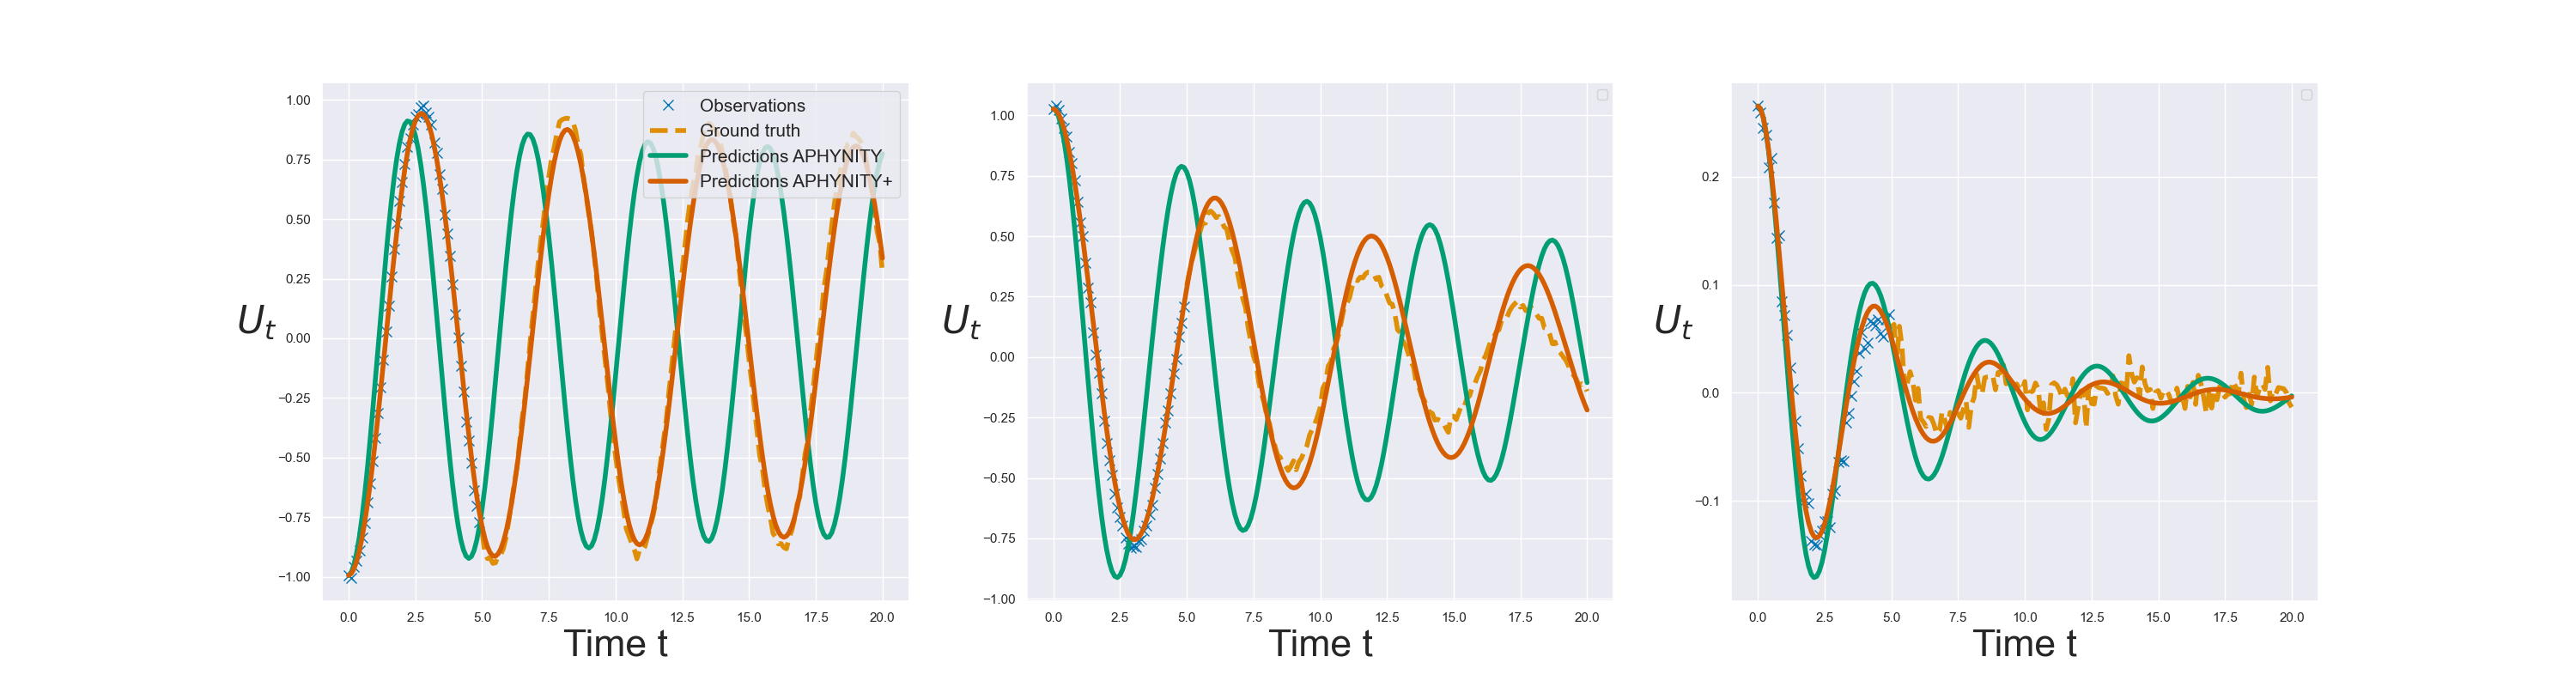
\includegraphics[width=.98\textwidth]{figures/pendulum_examples.png}
    \vspace{-1em}
    \caption{Comparison of the predictions made by APHYNITY and APHYNITY+ on the damped pendulum problem for 3 diverse test examples. It is important to mention that the support of the test distribution is disjoint from the training support. \textit{We clearly observe the beneficial effect of augmentation which lead to more accurate predictions.}}
    \label{fig:ood_pendulum}
\end{figure*}

\begin{figure*}
    \centering
    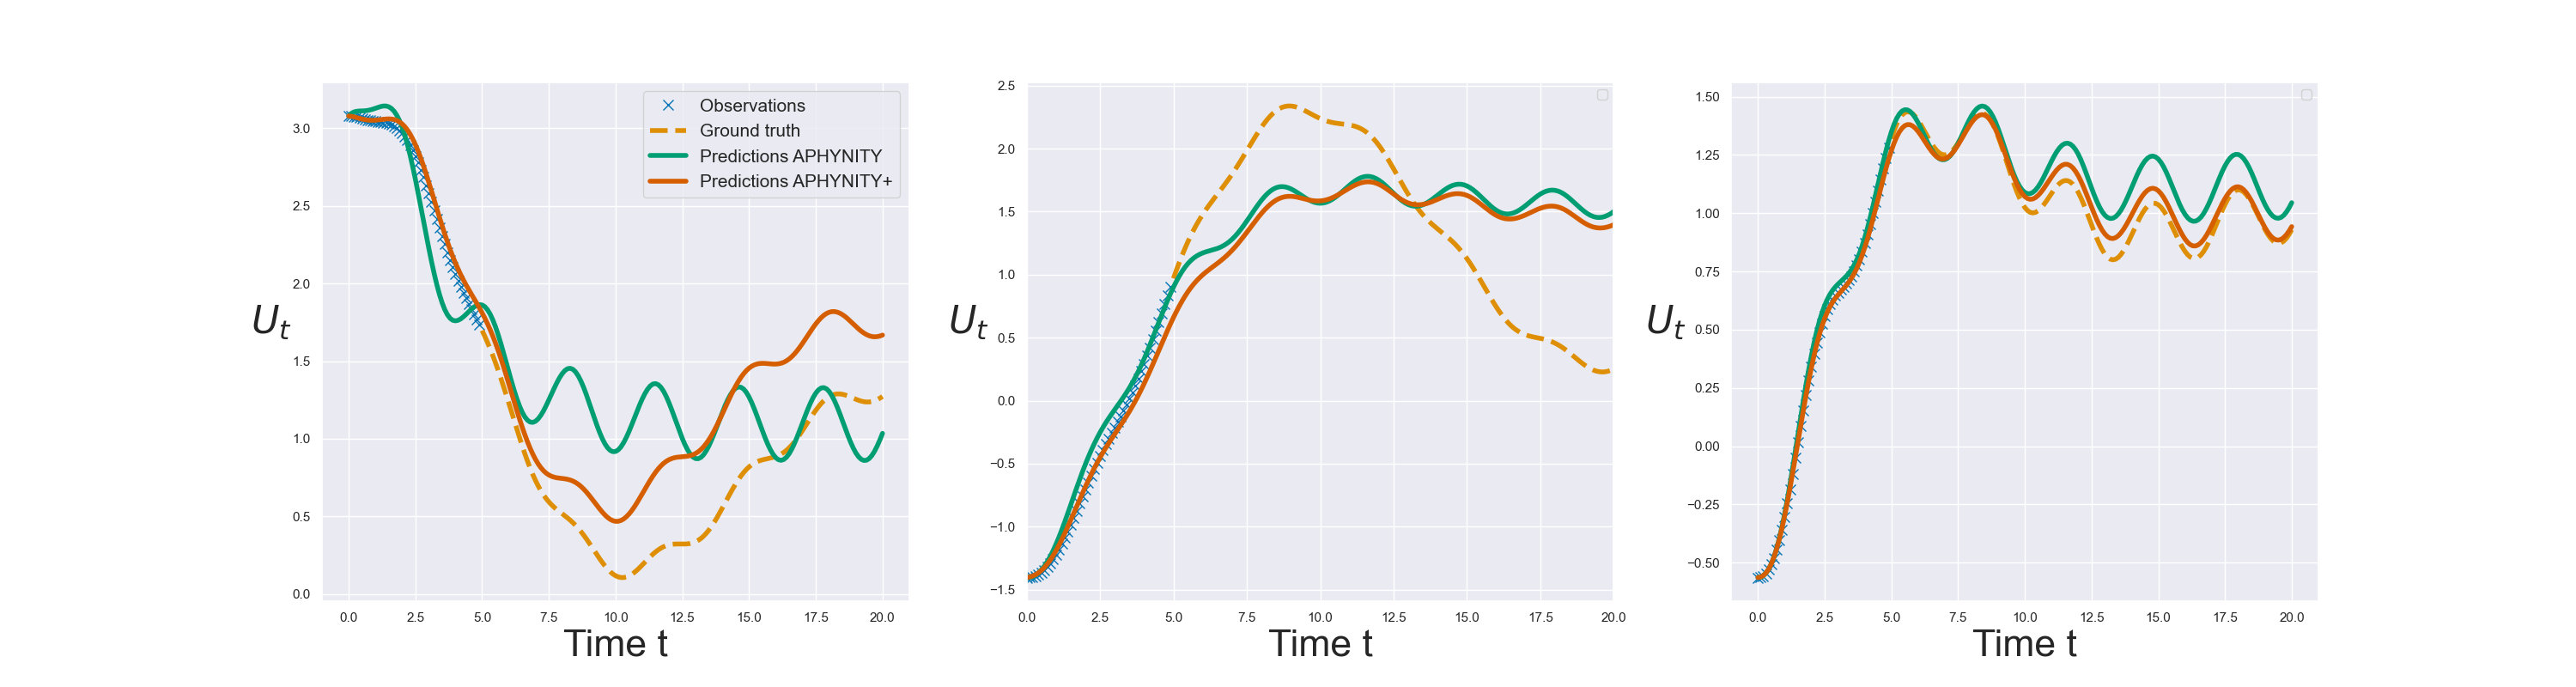
\includegraphics[width=.98\textwidth]{figures/RLC_examples.png}
    \vspace{-1em}
    \caption{Comparison of the predictions made by APHYNITY and APHYNITY+ on the RLC series problem for 3 diverse test examples. It is important to mention that the support of the test distribution is disjoint from the training support. \textit{We can perceive the beneficial effect of augmentation which lead to more accurate predictions in some cases. However both models are inaccurate. This indicates that the RLC series parameters are not easily identifiable, hence the generative model is not exact and augmentation is not as useful as for the diffusion and the pendulum.}}
    \label{fig:ood_RLC}
\end{figure*}
\subsection{On the effect of out of expertise shift}
The additional results in \figref{fig:za_ood_pendulum}, \figref{fig:za_ood_RLC} and \figref{fig:za_ood_diffusion} demonstrate that our augmentations is mostly always beneficial. Although the benefit of augmentation decreases with the gap between the support of the distributions of $z_a$ and train and test times, it still performs either better or on par with non-augmented HyL models.
\begin{figure*}
    \centering
    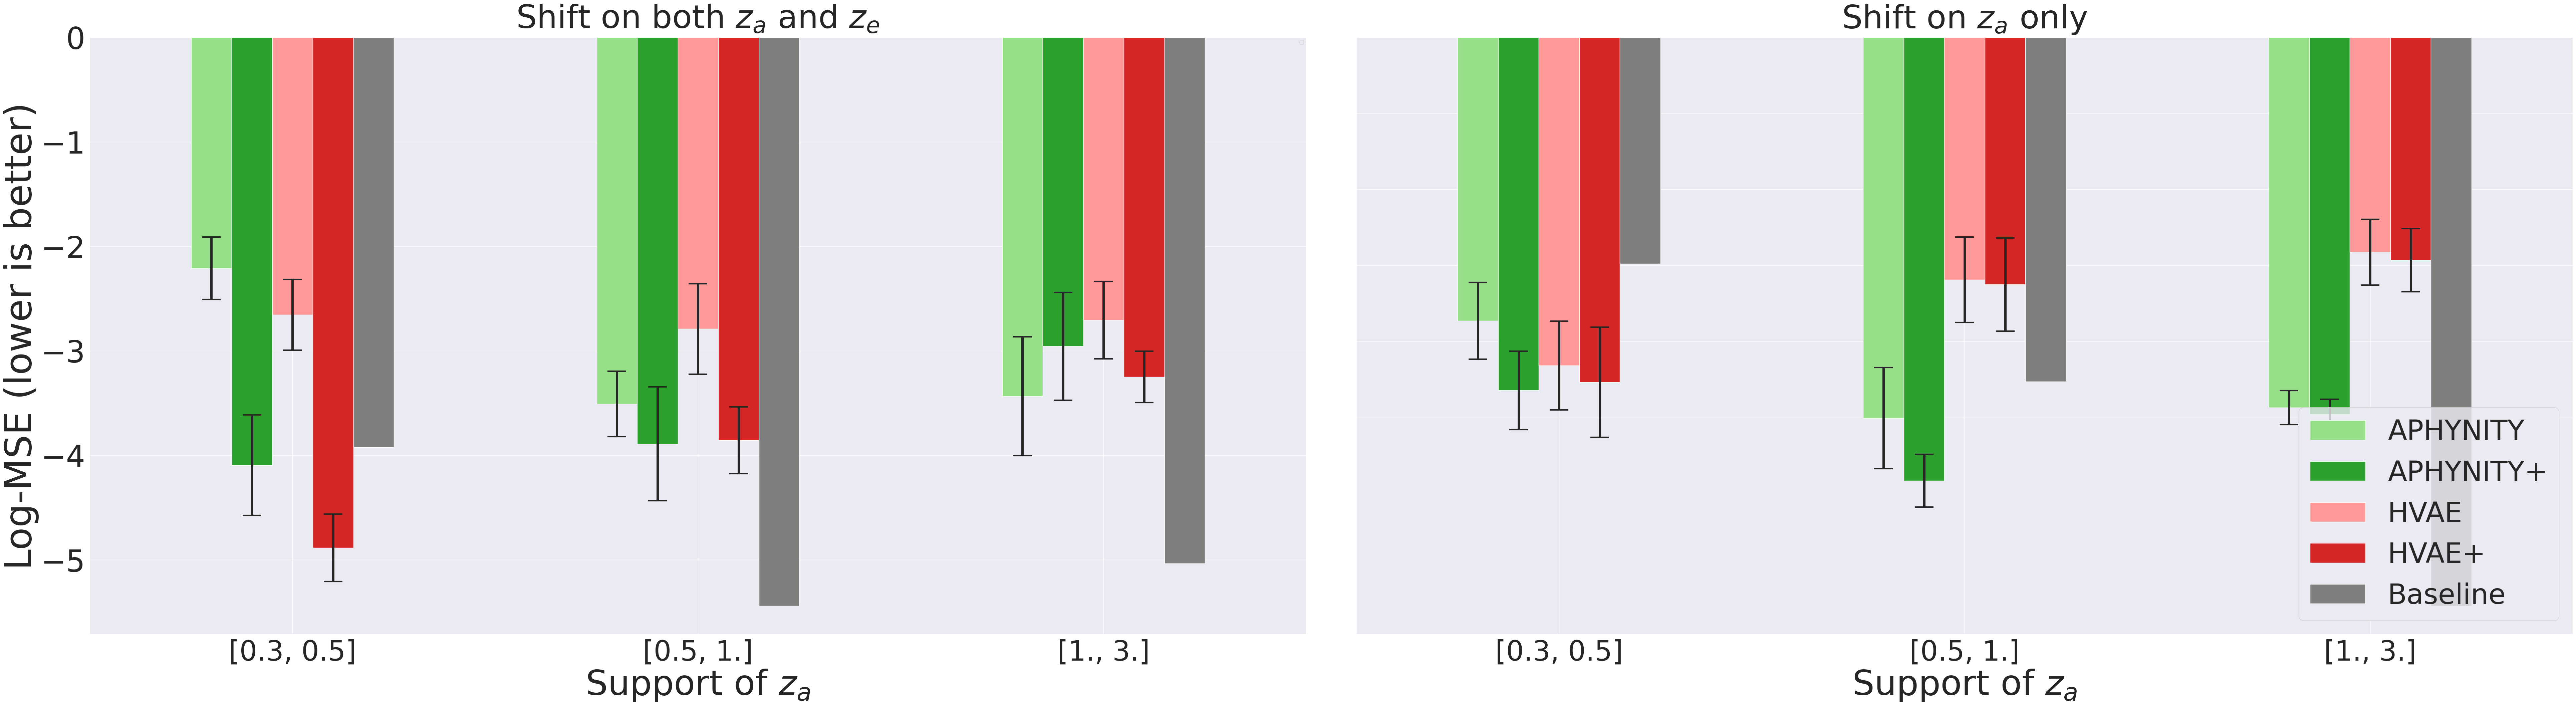
\includegraphics[width=.98\textwidth]{figures/results_log_mse_za_OOD_pendulum.png}
    \caption{\textbf{Damped pendulum.} Effect of a distribution shift on the latent variable $z_a$ of the interaction model. When the shift of $z_a$ is reasonable (less than $1$), the augmented models outperforms standard HyL even when the shift is only on $z_a$.}
    \label{fig:za_ood_pendulum}
\end{figure*}

\begin{figure*}
    \centering
    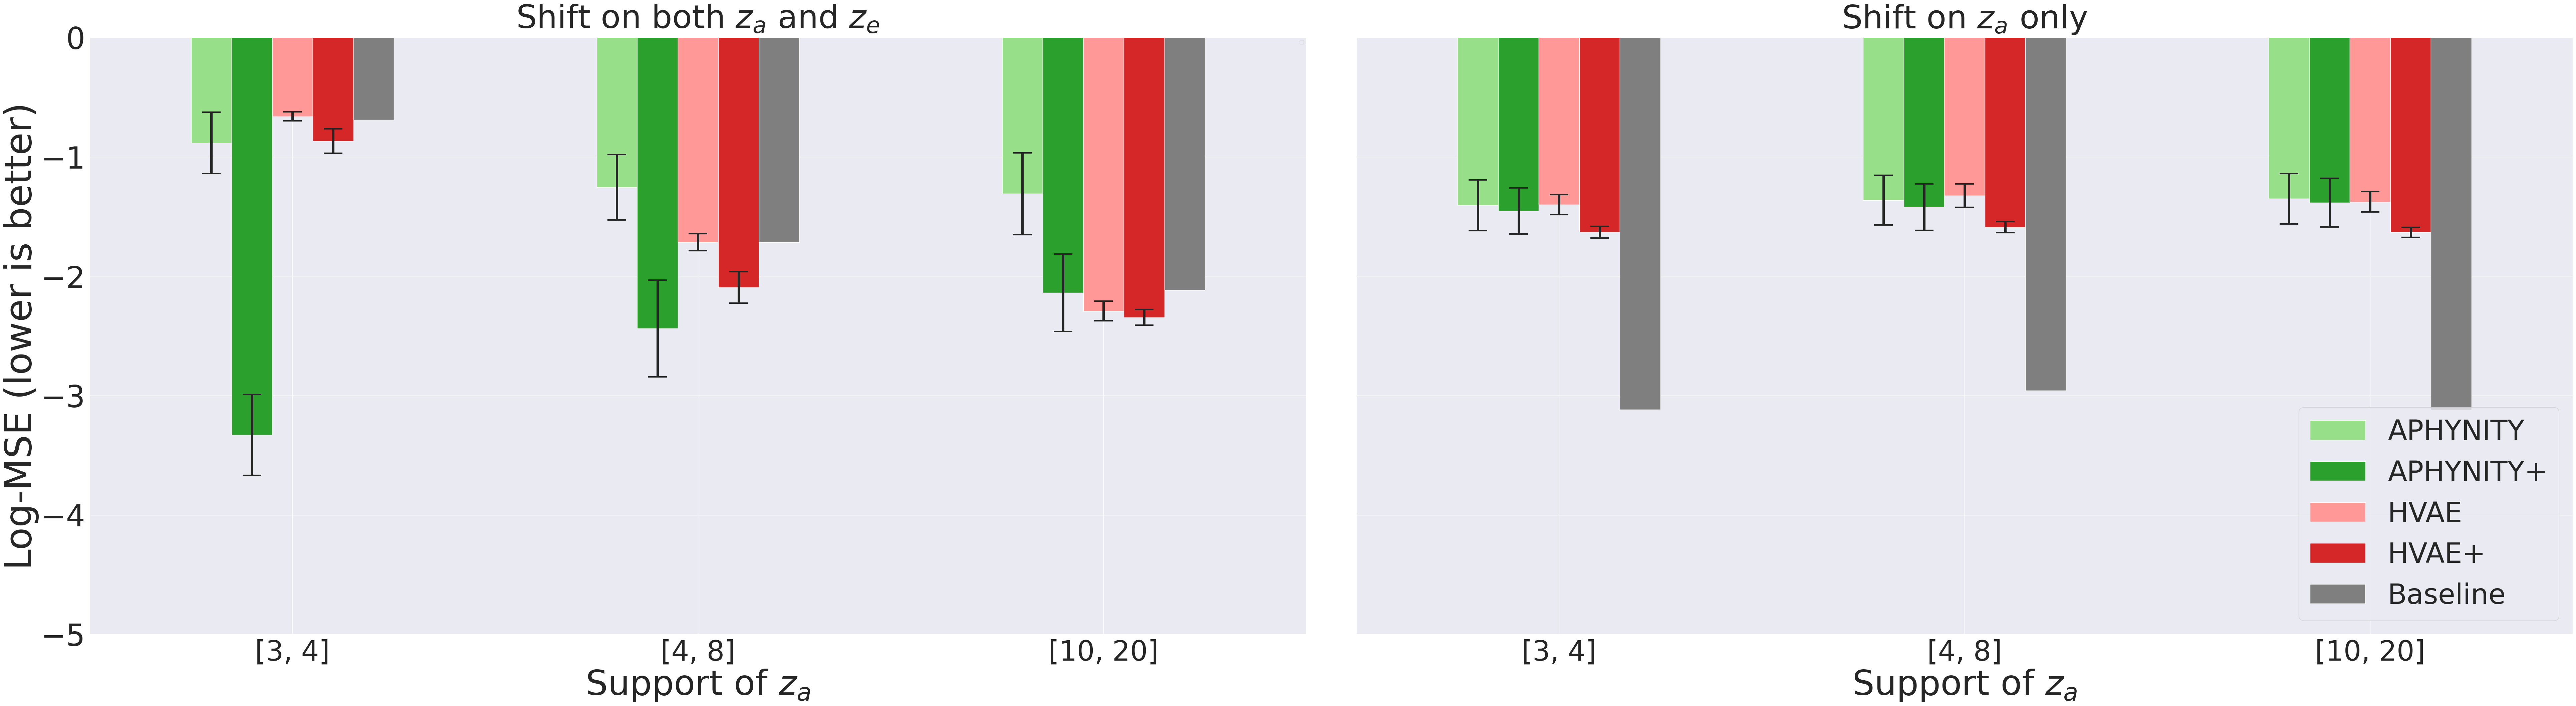
\includegraphics[width=.98\textwidth]{figures/results_log_mse_za_OOD_RLC.png}
    \caption{\textbf{RLC series.} Effect of a distribution shift on the latent variable $z_a$ of the interaction model. We observe that augmentation is always beneficial, even when the shift is only on $z_a$. As the dynamics of the RLC series systems depends on the values of all $3$ parameters $R, L, C$, we observe that some distribution shift can even lead to improved performance for the augmented models as for APHYNITY+ when $R \in \left[3, 4\right]$}
    \label{fig:za_ood_RLC}
\end{figure*}

\begin{figure*}
    \centering
    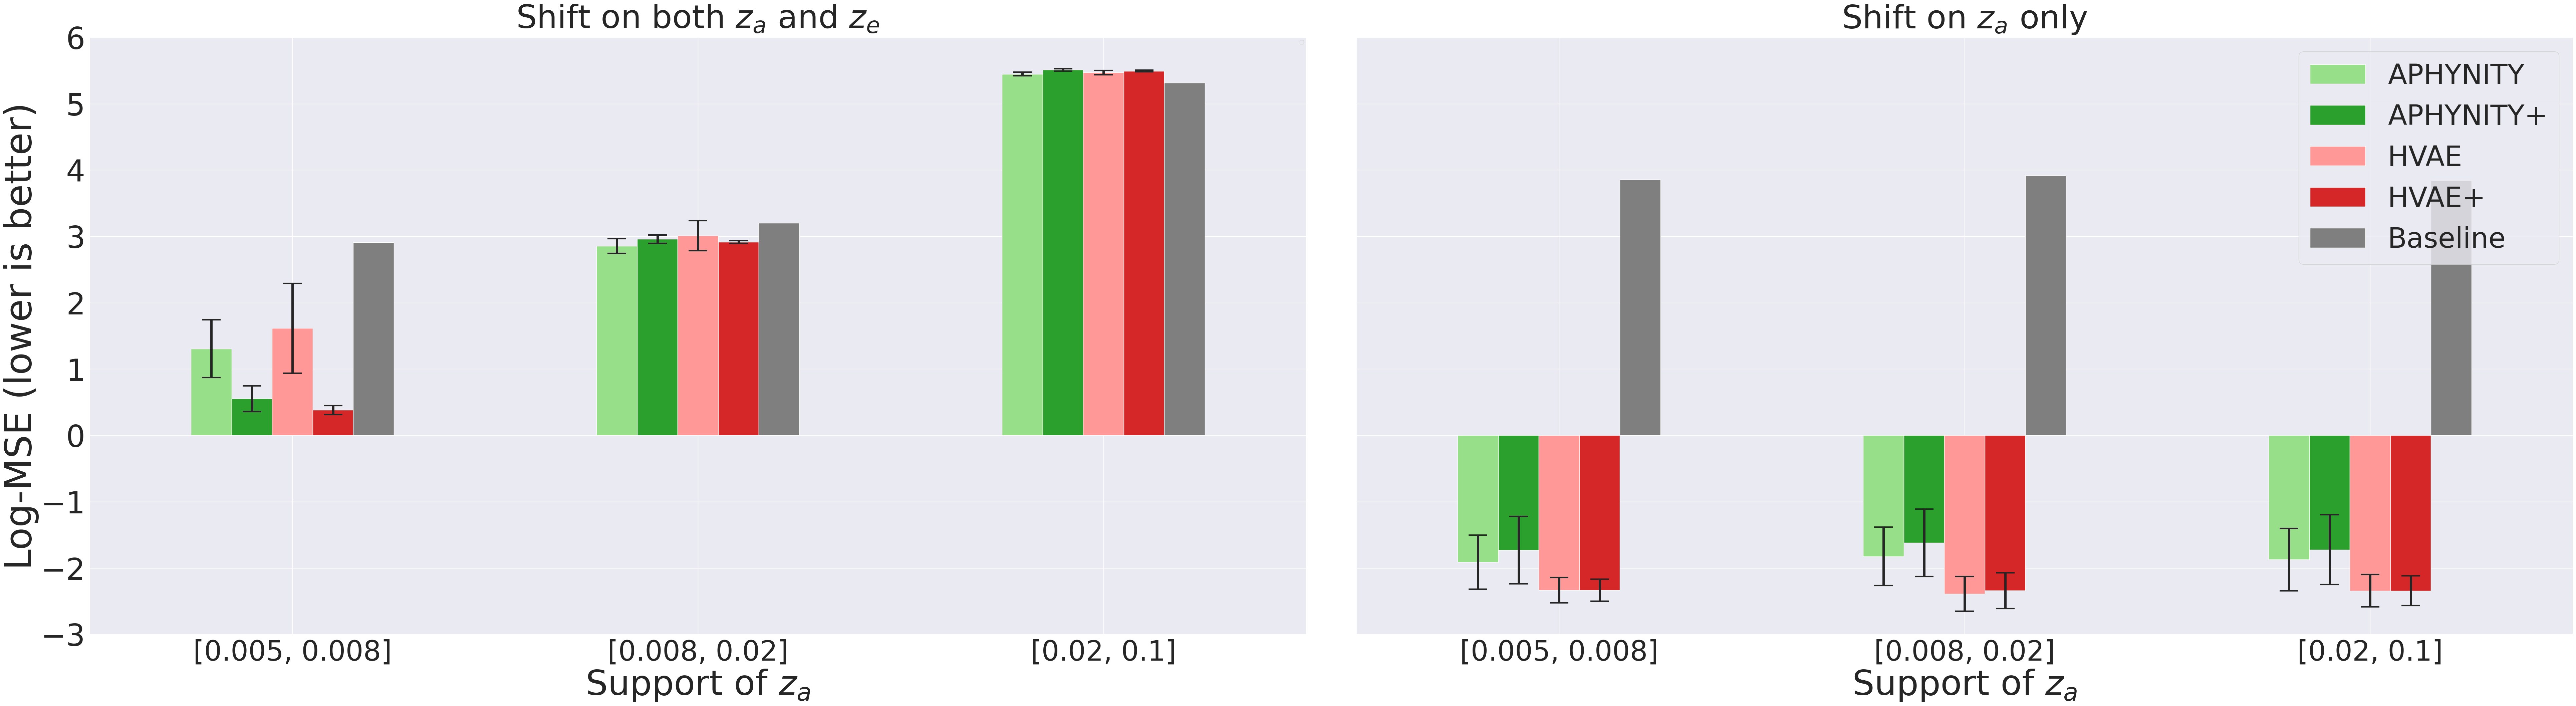
\includegraphics[width=.98\textwidth]{figures/results_log_mse_za_OOD_diffusion-2.png}
    \caption{\textbf{2D diffusion reaction.} Effect of a distribution shift on the latent variable $z_a$ of the interaction model. When the shift of $z_a$ is reasonable ($k < 0.008$), the augmented models outperforms standard HyL even when the shift is only on $z_a$.}
    \label{fig:za_ood_diffusion}
\end{figure*}

\end{document}